\documentclass[12pt,a4paper]{article}
\usepackage[utf8]{inputenc}
\usepackage[T1]{fontenc}
\usepackage{amsmath}
\usepackage{amsfonts}
\usepackage{amssymb}
\usepackage{graphicx}
\usepackage{geometry}
\usepackage{mathtools}
%\usepackage{diagrams}
\usepackage[document]{ragged2e}
\usepackage{wasysym}
\usepackage{pgfplots}
\usepackage{ mathrsfs }
\usepackage{braket}
\usepackage{simpler-wick}
\usepackage{tikz}
\usetikzlibrary{decorations.markings}
\usepackage{tikz-feynman}
\usepackage{subcaption}
\usepackage{bm}
\usepackage{slashed}
\usepackage{tensor}
\usepackage{hyperref}
\usepackage{float}
\usetikzlibrary{calc}
\tikzset{
	myarrow/.style={stealth-,shorten >=3pt,shorten <=3pt}
}
\pgfplotsset{
	lineplot/.style={
		black,
		dashed,
		very thin,
		samples y=0
	},
	coordinate line/.style={
		black,
		samples y=0
	},
	point/.style={
		only marks,
		mark=*,
		black,
		mark size=0.5pt
	}
}
\title{Topics in Mathematical Physics}
\author{Ben Karsberg}
\date{2021-22}
\newgeometry{vmargin={15mm}, hmargin={20mm,20mm}}
\numberwithin{equation}{section}
\DeclareMathSymbol{:}{\mathord}{operators}{"3A}
\begin{document}
	\maketitle
	\section{Preface}
	\begin{itemize}
		\item These notes were written up for the postgraduate masters course in mathematical physics at the University of Edinburgh
		\item The topic this year was 'Applications of Geometry in Physics'
		\item It was lectured by James Lucietti, who's notes are unfortunately only available on the Edinburgh intranet
		\item These notes were largely produced with those official notes as reference
		\item These notes were written primarily with myself in mind; it has some colloquialisms in it, and some topics are presented in the way I best understand them, and not necessarily the `best' way
		\item The notes are also exclusively bullet pointed because I find prose difficult to digest
		\item Any errors are most certainly mine and not James's - let me know at \href{mailto:benkarsberg@gmail.com}{benkarsberg@gmail.com} if you note any bad ones
		\item Generally, text in \textit{italic} is the definition of something the first time it shows up, and text in \textbf{bold} is something I think is important/want to remember/found tricky when writing these up
		\item Summation convention is implicit throughout this entire set of notes, unless explicitly stated otherwise
		\item Euclidean spatial vectors are denoted by e.g. $\mathbf{v}$, and 4-vectors are denoted by just $v=(v^{0},\mathbf{v})$
		\item The metric signature is $\eta_{\mu\nu}=\text{diag}(+1,-1,-1,-1)$ unless stated otherwise
		\item $\hbar=c=1$
		\item I hope these notes are helpful to someone who isn't me - enjoy!
	\end{itemize}
	\newpage
	\section{Differential Geometry Preliminaries}
	\begin{itemize}
		\item This course is all about geometry, almost entirely differential
		\item Differentiable geometry is a listed prerequisite for this course, but I haven't done any properly, with the exception of pseudo-Riemannian geometry in coordinate bases in a GR course last year
		\item Therefore, we need to set the scene
		\item The principal arena for differential geometry is a \textbf{differential manifold}:
		\begin{itemize}
			\item Informally, this is a set $M$ that locally looks like $\mathbb{R}^{n}$
			\item Formally, this is a topological space $M$ equipped with a collection of charts $\{(U_{\alpha},\phi_{\alpha})\}$ called an \textbf{atlas}, where $\{U_{\alpha}\}$ is an open cover of $M$ and $\phi_{\alpha}\;:\;U_{\alpha}\to V_{\alpha}\subset\mathbb{R}^{n}$ are homeomorphisms
		\end{itemize}
		\item The image we want in mind is something like this, generalised to $\mathbb{R}^{n}$ rather than just $\mathbb{R}^{2}$:
		\begin{figure}[H]
			\centering
		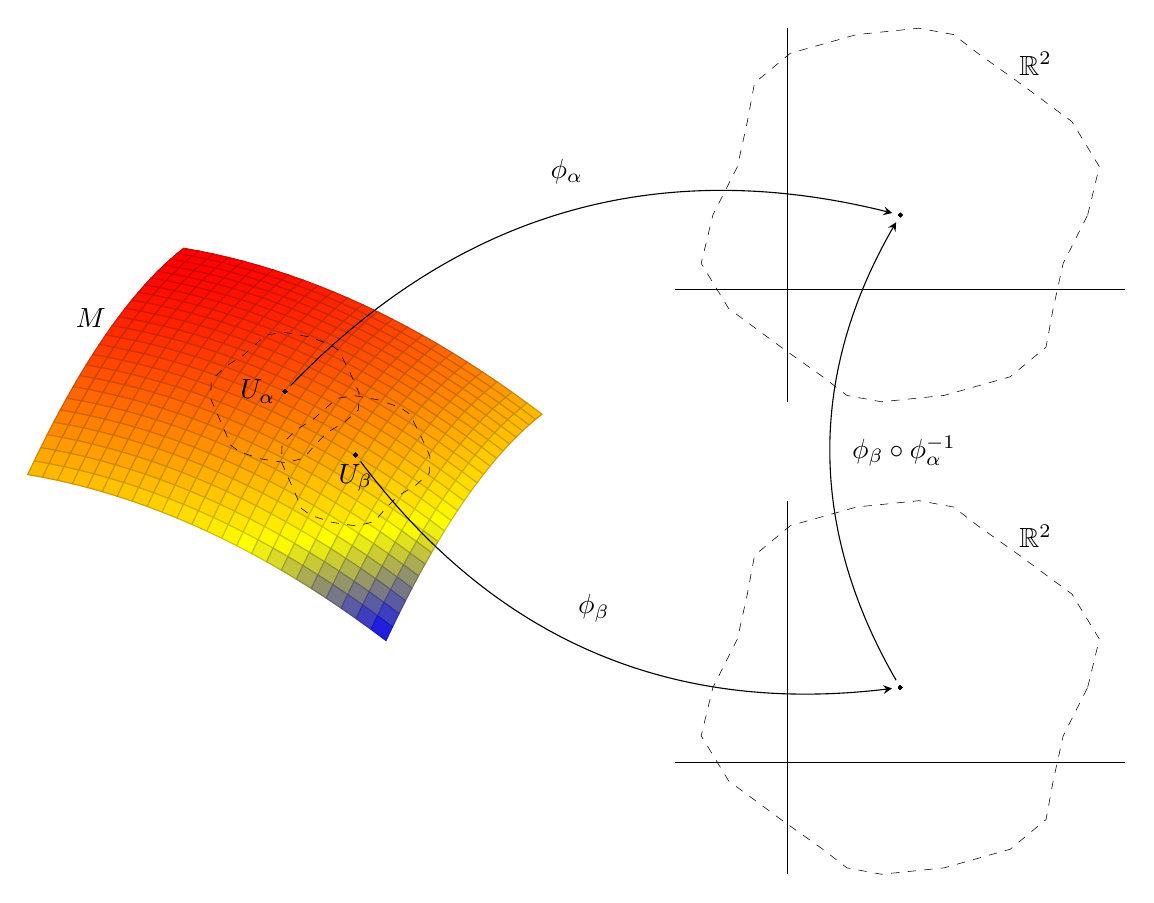
\begin{tikzpicture}
			\begin{axis}[
				name=mfd,
				axis lines=none,
				declare function={
					f(\x,\y)=10-(\x^2+\y^2);
				},
				declare function={
					c_x(\t)=(cos(\t)+(sin(5*\t)/10))/3+1;
				},
				declare function={
					c_y(\t)=(sin(\t))/2-1;
				},
				declare function={
					c_z(\t)=f(c_x(\t),c_y(\t));
				},
				declare function={
					x_0(\t)=-1.2;
				},
				declare function={
					x_1(\t)=0.8;
				}
				]
				\addplot3[surf,domain=0:2,domain y=-2:0,]{f(x,y)};
				\addplot3[lineplot,variable=t,domain=0:360] ({c_x(t)},{c_y(t)},{c_z(t)});
				\addplot3[lineplot,variable=t,domain=0:360] ({c_x(t)+0.7},{c_y(t)-0.7},{c_z(t)});
				%\addplot3[coordinate line,variable=t,domain=0:2] (t,{x_0(t)},{f(t,{x_0(t)})});
				%\addplot3[coordinate line,variable=t,domain=-2:0] ({x_1(t)},t,{f({x_1(t)},t)});
				\addplot3[point] (1,-1,{f(1,-1)}) coordinate (a);
				\addplot3[point] (1.7,-1.7,{f(1,-1)}) coordinate (c);
				%\addplot3[point](.5,{x_0(.5)},{f(.5,{x_0(.5)})}) coordinate (x_dot);
				%\addplot3[point]({x_1(-.5)},-.5,{f({x_1(-.5)},-.5)}) coordinate (y_dot);
			\end{axis}
				\draw (a) node [left] {$U_{\alpha}$};
				\draw (c) node [below] {$U_{\beta}$};
			\begin{axis}[
				at={($(mfd.north east)+(1cm,3cm)$)},
				anchor=north west,
				axis lines=none,
				declare function={
					c_x(\t)=(cos(\t)+(sin(5*\t)/10))/3+1;
				},
				declare function={
					c_y(\t)=(sin(\t))/2-1;
				},
				declare function={
					x_0(\t)=-1.2;
				},
				declare function={
					x_1(\t)=0.8;
				}
				]
				\addplot[lineplot,variable=t,domain=0:360]({c_x(t)},{c_y(t)});
				\addplot[point] (1,-1) coordinate (b);
				\addplot[coordinate line,variable=t,domain=0.6:1.4](t,{x_0(t)});
				\addplot[coordinate line,variable=t,domain=-1.5:-0.5]({x_1(t)},t);
				%\addplot[point](.8,-.5) coordinate (P1);
				%\addplot[point](.6,-1.2) coordinate (P2);
			\end{axis}
			\draw [myarrow] (b) to[bend right] node [above=7pt] {$\phi_{\alpha}$} (a);
			\draw (13,7.5) node [above] {$\mathbb{R}^{2}$};
			\draw (13,1.5) node [above] {$\mathbb{R}^{2}$};
			\draw (1,4.3) node [above] {$M$};
			%\draw [myarrow] (P1) to[bend left] ++(-1cm,1cm) node[above] {$(x \circ \gamma_{(1)})$};
			%\draw [myarrow] (P2) to[bend left] ++(-3cm,-1cm) node[above] {$(x \circ \gamma_{(0)})$};
			\begin{axis}[
				at={($(mfd.north east)+(1cm,-3cm)$)},
				anchor=north west,
				axis lines=none,
				declare function={
					c_x(\t)=(cos(\t)+(sin(5*\t)/10))/3+1;
				},
				declare function={
					c_y(\t)=(sin(\t))/2-1;
				},
				declare function={
					x_0(\t)=-1.2;
				},
				declare function={
					x_1(\t)=0.8;
				}
				]
				\addplot[lineplot,variable=t,domain=0:360]({c_x(t)},{c_y(t)});
				\addplot[point] (1,-1) coordinate (d);
				\addplot[coordinate line,variable=t,domain=0.6:1.4](t,{x_0(t)});
				\addplot[coordinate line,variable=t,domain=-1.5:-0.5]({x_1(t)},t);
			\end{axis}
			\draw [myarrow] (d) to[bend left] node [above=7pt] {$\phi_{\beta}$} (c);
			\draw [myarrow] (b) to[bend right] node [right=4pt] {$\phi_{\beta}\circ\phi_{\alpha}^{-1}$} (d);
		\end{tikzpicture}
		\end{figure}
		\item Essentially, a chart $(U,\phi)$ assigns coordinates to a point $p\in U$ given by $\phi(p)=(x^{1}(p),\ldots,x^{n}(p))$, usually written $\phi=\left(x^{i}\right)$
		\item Importantly, the \textbf{transition functions} $\phi_{\beta}\circ\phi_{\alpha}^{-1}\;:\;\phi_{\beta}(U_{\alpha}\cap U_{\beta})\to\phi_{\alpha}(U_{\alpha}\cap U_{\beta})$ should be $C^{\infty}(\mathbb{R}^{n})$ bijections between open subsets of $\mathbb{R}^{n}$ (see diagram)
		\item Essentially, all changes of coordinates are given by a smooth map
		\item The atlas allows us to define calculus on a manifold, and we can classify a hierarchy of objects on $M$:
		\begin{itemize}
			\item $C^{\infty}(M)$ is the set of all smooth functions on $M$, with the function of a standard commutative algebra
			\item The \textbf{tangent space} $T_{p}M$ at $p\in M$ is the $n$-dimensional vector space of directional derivatives at $p$; that is, the space of all $\mathbb{R}$-linear maps $X_{p}\;:\; C^{\infty}(M)\to\mathbb{R}$ obeying the Leibnitz/product rule
			\begin{equation}
				X_{p}(fg)=X_{p}(f)g(p)+f(p)X_{p}(g)
			\end{equation}
			for all $f,g\in C^{\infty}(M)$
			\item The elements $X_{p}\in T_{p}M$ are called \textbf{tangent vectors}; if we consider a smooth curve $\gamma\;:\;(a,a)\to M$ where $\gamma(0)=p$, we can define a tangent vector to the curve called the velocity $\dot{\gamma}\in T_{p}M$ by $\dot{\gamma}(f)=\left.\frac{d}{dt}f(\gamma(t))\right|_{t=0}$, and all tangent vectors arise like this
			\item A \textbf{vector field} $X\in\mathfrak{X}(M)$ is a smooth assignment to each $p\in M$ of a tangent vector $X_{p}\in T_{p}M$ (or more formally, a section of the \textbf{tangent bundle} $TM$)
			\item A \textbf{differential} $k$\textbf{-form} $\alpha_{p}$ at $p\in M$ is a smooth alternating multilinear map $\alpha_{p}\;:\;T_{p}M\times\ldots\times T_{p}M\to \mathbb{R}$
			\item The set of all $k$-forms is denoted $\Omega^{k}(M)$, where $\alpha(X_{1},\ldots,X_{k})\in C^{\infty}(M)$ and $X_{i}\in\mathfrak{X}(M)$
			\item In particular, 1-forms at $p$ are just dual vectors $\alpha_{p}\in T_{p}^{*}M$
			\item The \textbf{wedge produce} of $\alpha\in\Omega^{k}(M)$ and $\beta\in\Omega^{l}(M)$ is $\alpha\wedge\beta\in\Omega^{k+l}(M)$ where $\alpha\wedge\beta=(-1)^{kl}\beta\wedge\alpha$; in particular, for 1-forms we have
			\begin{equation}
				(\alpha\wedge\beta)(X,Y)=\alpha(X)\beta(Y)-\beta(X)\alpha(Y)
			\end{equation}
			\item The \textbf{exterior derivative} is a $\mathbb{R}$-linear map $d\;:\;\Omega^{k}(M)\to\Omega^{k+1}(M)$ satisfying $d^{2}=0$ and $d(\alpha\wedge\beta=(d\alpha)\wedge\beta +(-1)^{k}\alpha\wedge(d\beta)$
			\item The \textbf{interior derivative} $\iota_{X}\;:\;\Omega^{k}(M)\to\Omega^{k-1}(M)$ is defined by $\iota_{X}\alpha=\alpha(X,\ldots)$ for $X\in\mathfrak{X}(M)$
			\item In particular, if we regard a smooth function $f$ on $M$ as a 0-form, $(df)(X)=X(f)$
			\item \textbf{Tensors} and \textbf{tensor fields} of type $(r,s)$ are very similar to vectors and vector fields, acting as multilinear maps $T\;:\; T_{p}^{*}M\times\ldots T_{p}^{*}M\times T_{p}M\times\ldots T_{p}M\to\mathbb{R}$
			\item The derivative of a smooth map $\phi\;:\;M\to N$ is called the \textbf{push-forward map} $\phi_{*}\;:\;T_{p}M\to T_{\phi(p)}N$ given by
			\begin{equation}
				(\phi_{*}X_{p})(f)=X_{p}(f\circ\phi)
			\end{equation} 
			where $f\in C^{\infty}(N)$
			\item Similarly, the \textbf{pull-back} is $\phi^{*}\;:\;T_{\phi(p)}^{*}N\to T_{p}^{*}M$ given by
			\begin{equation}
				(\phi^{*}\alpha_{\phi(p)})(X_{p})=\alpha_{\phi(p)}(\phi_{*}X_{p})
			\end{equation}
			\item A smooth bijection $\phi\;:\;M\to N$ is called a \textbf{diffeomorphism}, and for a diffeomorphism we have $(\phi^{-1})_{*}=\phi^{*}$
			\item The \textbf{flow} of a vector field $X$ is a 1-parameter group of diffeomorphisms; i.e. a family $\phi_{t}\;:\;M\to M$ such that $\phi_{t+s}=\phi_{t}\circ\phi_{s}$ for all real $t,s$
			\item In particular, the integral curve of $X$ through $p\in M$ is given by $\phi_{t}(p)$ so $X_{p}(f)=\frac{d}{dt}f(\phi_{t}(p))|_{t=0}$
			\item The \textbf{Lie derivative} of a tensor field $T$ along a vector field $X$ is
			\begin{equation}
				\mathcal{L}_{X}T=\left.\frac{d}{dt}(\phi_{t}^{*}T)\right|_{t=0}
			\end{equation}
			where $\phi_{t}$ is the flow of $X\in\mathfrak{X}(M)$
			\item In particular, we have $\mathcal{L}_{X}f=X(f)$ for $f\in C^{\infty}(M)$; $\mathcal{L}_{X}Y=[X,Y]$ for $Y\in\mathfrak{X}(M)$; $\mathcal{L}_{X}\alpha=(d\iota_{X}+\iota_{X}d)\alpha$ for $\alpha\in\Omega^{k}(M)$
		\end{itemize}
		\item Suppose we have a local basis $\{e_{a}\;|\;a=1,\ldots,n\}$ of vectors; we can then expand a vector field as $X=X^{a}e_{a}$ where $X^{a}$ are the components
		\item The dual basis is $\{f^{a}\;|\;a=1,\ldots,n\}$ defined by $f^{a}(e_{b})=\delta^{a}_{b}$; differential 1-forms can then be expanded as $\alpha=\alpha_{a}f^{a}$ where $\alpha_{a}=\alpha(e_{a})$ are the components
		\item More generally, a $k$-form can be expanded as $\alpha=\frac{1}{k!}\alpha_{a_{1}\ldots a_{k}}f^{a_{1}}\wedge\ldots\wedge f^{a_{k}}$ where $\alpha_{a_{1}\ldots a_{k}}=\alpha(e_{a_{1}},\ldots,e_{a_{k}})$
		\item This generalises to tensors in the expected way
		\item In particular, a chart $(U,\phi)$ where $\phi=x^{i}$ defines a basis of $T_{p}M$ called the \textbf{coordinate basis}, $\left(\frac{\partial}{\partial x^{i}}\right)_{p}$
		\item In this basis, any vector field can be expanded as $X=X^{i}\frac{\partial}{\partial x^{i}}$ where $X^{i}=X(x^{i})$ are smooth functions on $U$
		\item Similarly, the dual basis of $T_{p}^{*}M$ is $(dx^{i})_{p}$, where 1-forms can be expanded as $\alpha=\alpha_{i}dx^{i}$, and this can be expanded to a basis for $k$-forms by $dx^{i_{1}}\wedge\ldots\wedge dx^{i_{k}}$ where $i_{1}<\ldots<i_{k}$
	\end{itemize}
\newpage
	\section{Symplectic Geometry and Classical Mechanics}
	\begin{itemize}
		\item To motivate what follows, consider a classical Hamiltonian system with phase space $\mathbb{R}^{2n}$ and canonical coordinates $(\mathbf{p},\mathbf{q})$
		\item Hamilton's equations for the time-evolution of the system are
		\begin{equation}
			\dot{\mathbf{p}}=-\frac{\partial H}{\partial \mathbf{q}},\quad\dot{\mathbf{q}}=\frac{\partial H}{\partial \mathbf{p}}
		\end{equation}
		where $H$ is the Hamiltonian
		\item This can be rewritten in matrix form:
		\begin{equation}
			\begin{pmatrix}\dot{\mathbf{p}}\\\dot{\mathbf{q}}\end{pmatrix}=\begin{pmatrix}0&I_{n}\\-I_{n}&0\end{pmatrix}\begin{pmatrix}\dfrac{\partial H}{\partial \mathbf{q}}\\[1em]\dfrac{\partial H}{\partial \mathbf{p}}\end{pmatrix}\iff \dot{\mathbf{x}}=\Omega^{-1}\nabla_{\mathbf{x}}H
		\end{equation}
		where
		\begin{equation}
			\Omega=\begin{pmatrix}
				0&-I_{n}\\I_{n}&0
			\end{pmatrix}\quad\text{and}\quad\mathbf{x}=\begin{pmatrix}
			\mathbf{p}\\\mathbf{q}
		\end{pmatrix}
		\end{equation}
		is implicit
		\item As we shall see, this is the canonical example of a symplectic vector space
	\end{itemize}
	\subsection{Symplectic Vector Spaces}
	\begin{itemize}
		\item A \textbf{symplectic vector space} is a pair $(V,\omega)$, where $V$ is a $2n$-dimensional real vector space, and $\omega\,:\,V\times V\to \mathbb{R}$ is a bilinear form satisfying:
		\begin{enumerate}
			\item \textit{Skew-symmetry}: $\omega(v,w)=-\omega(w,v),\,\forall v,w\in V$
			\item \textit{Non-degeneracy}: $\omega(v,w)=0\,\forall v\in V \implies w=0$
		\end{enumerate}
		\item $\omega$ is called a \textbf{symplectic structure} on $V$
		\item Contrasting $\omega$ with the standard Euclidean inner product, the only real difference is skew vs non-skew symmetry
		\item In physics, we usually need a basis to work in - defining the arbitrary basis $\{e_{a}\,|\,a=1,\ldots, 2n\}$, the components of $\omega$ are given by the usual $\omega_{ab}=\omega(e_{a},e_{b})$
		\item From this, it follows that $\omega_{ab}$ is an antisymmetric matrix
		\item Moreover, non-degeneracy of $\omega$ is equivalent to
		\begin{equation}
			\omega_{ab}w^{b}\implies w^{a}=0
		\end{equation}
		which just means $\omega_{ab}$ is invertible
		\item \textbf{Example:} the canonical example of a symplectic vector space is $V=\mathbb{R}^{2n}$ and $\omega(\mathbf{v},\mathbf{w})=\mathbf{v}^{T}\Omega\mathbf{w}$, with $\Omega$ as defined in the introduction:
		\begin{equation}
			\Omega=\begin{pmatrix}
				0&I_{n}\\-I_{n}&0
			\end{pmatrix}
		\end{equation}
		\item We now show that, in fact, all symplectic vector spaces are isomorphic to this example
		\item \textbf{Theorem:} any symplectic vector space $(V,\omega)$ has a \textbf{symplectic basis} $\{e_{i},f_{i}\,|\,i=1,\ldots,n\}$ defined by
		\begin{equation}
			\omega(e_{i},e_{j})=\omega(f_{i},f_{j})=0\quad\text{and}\quad\omega(e_{i},f_{j})=\delta_{ij}
		\end{equation}
		\item \textbf{Proof:} by induction
		\begin{itemize}
			\item For the $n=1$ case, pick an arbitrary vector $0\neq e_{1}\in V$
			\item By non-degeneracy, $\exists f_{1}\in V$ such that $\omega(e_{1},f_{1})\neq 0$, and we can rescale so that $\omega(e_{1},f_{1})=1$
			\item Then, by skew-symmetry, we see $\omega(e_{1},e_{1})=\omega(f_{1},f_{1})=0$ as required
			\item Assume the hypothesis holds for $n=k\geq1$, and consider the $n=k+1$ case
			\item By the same procedure that we used for the base case, we can construct $e_{1}$ and $f_{1}$
			\item Then, define the \textit{skew-orthogonal complement}:
			\begin{equation}
				W=\{w\in V\,|\,\omega(w,e_{1})=\omega(w,f_{1})=0\}
			\end{equation}
			\item $W$ has dimension $2k$, and we now wish to show that it is a symplectic vector space
			\item First note that any $v\in V$ can be uniquely decomposed as $v=u+w$, where $u\in\text{span}(e_{1},f_{1})$ and $w\in W$
			\item Then consider $\omega|_{W}$, i.e. the symplectic structure restricted to $W$; pick $\tilde{w}\in W$, then:
			\begin{equation}
				\begin{aligned}
					\omega(\tilde{w},w)=0,\;\forall w\in W &\implies \omega(\tilde{w},v)=0, \;\forall v\in V \quad&\text{(by decomposition above)}\\
					&\implies \tilde{w}=0\quad&\text{(by non-degeneracy)}
				\end{aligned}
			\end{equation}
			\item $\omega|_{W}$ clearly inherits skew-symmetry from $\omega$, so it is a symplectic form, and so $W$ is indeed a symplectic vector space
			\item By induction the conclusion follows $\blacksquare$
		\end{itemize}
		\item Explicitly, this means in the symplectic basis $\omega_{ab}=\Omega_{ab}$, establishing the isomorphism 
		\item The next result shows a radical departure from Euclidean geometry in these spaces
		\item \textbf{Theorem:} let $(V,\omega)$ be a $2n$-dimensional symplectic vector space, and $W\subset V$ a \textit{null subspace} so $\omega|_{W}=0$. Then $\dim{W}\leq n$
		\item \textbf{Proof:}
		\begin{itemize}
			\item By the earlier theorem, we can assume $V=\mathbb{R}^{2n}$ and $\omega=\Omega$
			\item Then, $W$ is a null space iff $W\bot \Omega W$, where this is with respect to the Euclidean norm $\mathbf{w}\cdot \mathbf{v}=\mathbf{w}^{T}\mathbf{v}$
			\item Therefore, we have
			\begin{equation}
				\dim{W}+\dim{\Omega W}\leq 2n
			\end{equation}
			\item However, $\Omega$ is invertible so $\dim{W}=\dim{\Omega W}$, so we are done $\blacksquare$
		\end{itemize}
		\item We now want to rewrite the symplectic structure in a symplectic basis, but in a more useful way
		\item Define the dual symplectic basis $\{e_{*}^{i},f_{*}^{i}\,|\,i=1,\ldots,n\}$ of $V^{*}$, so specifically:
		\begin{equation}
			e_{*}^{i}(e_{j})=f_{*}^{i}(f_{j})=\delta^{i}_{j},\quad e_{*}^{i}(f_{j})=f_{*}^{i}(e_{j})=0
		\end{equation}
		\item Then, the basis of 2-forms is given by the set
		\begin{equation}
			\{e_{*}^{i}\wedge e_{*}^{j},\,e_{*}^{i}\wedge f_{*}^{j},\,f_{*}^{i}\wedge f_{*}^{j}\}
		\end{equation}
		as usual
		\item We therefore claim that
		\begin{equation}
			\omega = e_{*}^{i}\wedge f_{*}^{i}
		\end{equation}
		with summation convention implied
		\item We can easily verify this by its action on basis elements:
		\begin{equation}
			\omega(e_{a},e_{b})=(e_{*}^{i}\wedge f_{*}^{i})(e_{a},e_{b})=e_{*}^{i}(e_{a})f_{*}^{i}(f_{b})-e_{*}^{i}(f_{b})f_{*}^{i}(e_{a})=\delta^{i}_{a}\delta^{i}_{b}=\delta_{ab}
		\end{equation}
		\item More generally, consider the $k$-fold wedge product $\omega^{k}$
		\item We have $\omega^{k}=0$ for $k>n$ as $\omega^{n}$ is the highest ranked form on $V$, which has dimension $2n$
		\item \textbf{Lemma:} let $(V,\omega)$ be a $2n$-dimensional symplectic vector space. Then, in a symplectic basis we have
		\begin{equation}
			\omega^{n}=n!e_{*}^{1}\wedge f_{*}^{1}\wedge\ldots\wedge e_{*}^{n}\wedge f_{*}^{n}
		\end{equation}
		\item \textbf{Proof:} by induction (not given, but it's not hard - future Ben, just try and do it yourself for revision xx)
	\end{itemize}
	\subsection{Symplectic Manifolds and the Cotangent Bundle}
	\begin{itemize}
		\item A \textbf{symplectic manifold} is a pair $(M,\omega)$ where $M$ is a 2-dimensional smooth manifold, and $\omega\in\Omega^{2}(M)$ is a 2-form satisfying:
		\begin{enumerate}
			\item $d\omega=0$ (closed)
			\item $\omega(X,Y)=0\;\forall X\in\mathfrak{X}(M)\implies Y=0$ (non-degenerate)
		\end{enumerate}
		\item $\omega$ is called a \textbf{symplectic form}
		\item Note that if $(M,\omega)$ is a symplectic manifold, then $(T_{x}M,\omega_{x})$ is a symplectic vector space at all points $x\in M$
		\item \textbf{Example:} let $M=\mathbb{R}^{2n}$ with coordinates $(p_{i},q_{i}),\,i=1,\ldots,n$, and $\omega=dp_{i}\wedge dq_{i}$ (summation implied)
		\begin{itemize}
			\item $\omega=d(p_{i}dq_{i})$, so it is exact and hence closed
			\item Consider the components of $\omega$ in the coordinate basis $(\partial/\partial p_{i},\partial/\partial q_{i})$; we find
			\begin{equation}
				\begin{aligned}
					\omega\left(\frac{\partial}{\partial p_{j}},\frac{\partial}{\partial p_{k}}\right)&=\omega\left(\frac{\partial}{\partial q_{j}},\frac{\partial}{\partial q_{k}}\right)=0\\
					\omega\left(\frac{\partial}{\partial p_{j}},\frac{\partial}{\partial q_{k}}\right)&=dp_{i}\left(\frac{\partial}{\partial p_{j}}\right)dq_{i}\left(\frac{\partial}{\partial q_{k}}\right)=\delta_{ij}\delta_{ik}=\delta_{jk}
				\end{aligned}
			\end{equation}
			so in particular, $\omega_{ij}=\Omega_{ij}$ in this basis and is non-degenerate
			\item In particular, this means $\omega$ is a symplectic form and that $(\partial/\partial p_{i},\partial/\partial q_{i})$ is a symplectic basis at every point
		\end{itemize}
		\item \textbf{Theorem:} any symplectic manifold $(M,\omega)$ of dimension $2n$ is orientable with volume form $\omega^{n}$
		\item \textbf{Proof:}
		\begin{itemize}
			\item A manifold is \textbf{orientable} if there is a consistent definition of clockwise and anti-clockwise (e.g. a Mobius strip would be non-orientable), and a \textbf{volume form} is a highest-rank differentiable form on the manifold (of rank equal to the dimension of the manifold)
			\item One characterisation of orientability is that a manifold is orientable if and only if there exists a nowhere vanishing top-ranked differential form/volume form
			\item Therefore, if we can show $\omega^{n}=\omega\wedge\ldots\wedge\omega$ is nowhere vanishing, we are done
			\item At each $x\in M$, $(T_{x}M,\omega_{x})$ is a symplectic vector space
			\item But we know that in symplectic vector spaces
			\begin{equation}
				\omega_{x}^{n}=n!e_{*}^{1}\wedge f_{*}^{1}\wedge\ldots\wedge e_{*}^{n}\wedge f_{*}^{n}
			\end{equation}
			which is nowhere vanishing $\blacksquare$
		\end{itemize}
		\item \textbf{Example:} consider the manifold given by the unit 2-sphere $M=S^{2}=\{\mathbf{x}\in\mathbb{R}^{3}\,|\,\lvert\mathbf{x}\rvert=1\}$
		\begin{itemize}
			\item The tangent space at $\mathbf{x}$ is $T_{\mathbf{x}}S^{2}=span(\mathbf{x})^{\perp}$
			\item The volume form at this point is given by
			\begin{equation}
				\omega_{\mathbf{x}}(\mathbf{V},\mathbf{w})=\mathbf{x}\cdot (\mathbf{v}\times\mathbf{w})
			\end{equation}
			for $\mathbf{v},\mathbf{w}\in T_{\mathbf{x}}S^{2}$
		\end{itemize}
	\end{itemize}
	\subsubsection{The Cotangent Bundle}
	\begin{itemize}
		\item The following discussion is why symplectic manifolds arise in classical mechanics
		\item Suppose $Q$ is a $2n$-dimensional smooth manifold; its \textbf{cotangent bundle} is defined by
		\begin{equation}
			T^{*}Q=\{(p_{x},x)\,|\,p_{x}\in T_{x}^{*}Q,\,x\in Q\}
		\end{equation}
		which we think of as the set of all points $x$ paired with all their covectors (one-forms)
		\begin{itemize}
			\item The cotangent bundle is a $2n$-dimensional manifold
			\item To show this, consider the chart on $Q$ given by $\phi(x)=(q_{i}(x))$, containing $x\in Q$
			\item We can see that $\Phi(p_{x},x)=(p_{i}(x),q_{i}(x))$ is then a chart on $T^{*}Q$, where $p_{i}$ are the components of $p_{x}=p_{i}(x)(dq_{i})_{x}$
			\item To check the transition functions are smooth, consider the projection $\pi\,:\,T^{*}Q\to Q,\;(p_{x},x)\to x$; this is smooth and surjective, and the inverse projection has image $\pi^{-1}(x)=T_{x}^{*}Q$
			\item Therefore, $\phi\circ \pi\circ\Phi^{-1}(p_{i}(x),q_{i}(x))=(q_{i}(x))$ is smooth
		\end{itemize}
		\item \textbf{Theorem:} $T^{*}Q$ has a symplectic form $\omega$, given in the above chart by
		\begin{equation}
			\omega=dp_{i}\wedge dq_{i}
		\end{equation}
		\item \textbf{Proof:}
		\begin{itemize}
			\item Recall that the derivative of a smooth map $\phi\,:\,M \to N$ is the push-forward map $\phi_{*}\,:\,T_{p}M\to T_{\phi(p)}N$, given by
			\begin{equation}
				(\phi_{*}X_{p})(f)=X_{p}(f\o\phi)
			\end{equation}
			\item Moreover, the pull-back of $\phi$ is $\phi^{*}\,:\,T_{\phi(p)}^{*}N\to T_{p}^{*}M$, given by
			\begin{equation}
				(\phi^{*}\alpha_{\phi(p)})(X_{p})=\alpha_{\phi(p)}(\phi_{*}X_{p})
			\end{equation}
			\item The projector above is a smooth map of this form, so its derivative is the push-forward $\pi_{*}\,:\,T_{(p_{x},x)}(T^{*}Q)\to T_{x}Q$
			\item We now define $\theta_{(p_{x},x)}\in T^{*}_{(p_{x},x)}(T^{*}Q)$, given by
			\begin{equation}
				\theta_{(p_{x},x)}(\xi)=p_{x}(\pi_{*}\xi) ,\quad \forall \xi \in T_{(p_{x},x)}(T^{*}Q)
			\end{equation}
			so $\theta_{(p_{x},x)}=\pi^{*}p_{x}$ is the pull-back of $p_{x}$ under $\pi$, meaning $\theta\in \Omega^{1}(T^{*}Q)$ is a one-form on $T^{*}Q$
			\item Define $\omega = d\theta\in\Omega^{2}(T^{*}Q)$, which is clearly closed since it is exact
			\item To show non-degeneracy, we check the components of $\theta$ in the chart $\Phi=(p_{i},q_{i})$ above of $T^{*}Q$, defined by chart $\phi=(q_{i})$ of Q
			\item We find first that
			\begin{equation}
				\theta\left(\frac{\partial}{\partial q_{i}}\right)=p\left(\pi_{*}\frac{\partial}{\partial q_{i}}\right)
			\end{equation}
			and note in particular that
			\begin{equation}
				\begin{aligned}
					\left(\pi_{*}\frac{\partial}{\partial q_{i}}\right)(f)&=\frac{\partial}{\partial q_{i}}(f\circ\pi)\\&=\frac{d}{dt}f\circ\pi\circ\Phi^{-1}(p_{1},\ldots,p_{n},q_{1},\ldots,q_{i}+t,\ldots,q_{n})\vert_{t=0}\\&=\frac{d}{dt}f\circ\phi^{-1}(q_{1},\ldots,q_{i}+t,\ldots,q_{n})\vert_{t=0}\\&=\frac{\partial}{\partial q_{i}}(f)
				\end{aligned}
			\end{equation}
			for all $f\in C^{\infty}(Q)$
			\item Therefore, $\theta(\partial/\partial q_{i})=p(\partial/\partial q_{i})=p_{i}$
			\item A similar calculation finds $\pi_{*}\partial/\partial p_{i}=0$, so $\theta(\partial/\partial p_{i})=0$
			\item Therefore, $\theta=p_{i}dq_{i}$ in this chart $\blacksquare$
		\end{itemize}
		\item This has a very clear link to classical mechanics: $Q$ is the configuration space, and $T^{*}Q$ is the phase space
		\item A symplectic manifold also induces a rather natural isomorphism between the tangent and cotangent space
		\item Specifically, this isomorphism is between the tangent space at each point and its dual
		\item \textbf{Theorem:} let $(V,\omega)$ be a symplectic vector space; then there is a `natural' isomorphism called the musical isomorphism $V\equiv V^{*}$
		\item \textbf{Proof:}
		\begin{itemize}
			\item Let $\xi\in V$; we define the linear map $\flat\,:\,V\to V^{*}$ by
			\begin{equation}
				\xi^{\flat}(\eta)=\omega(\eta,\xi),\quad\forall\eta\in V
			\end{equation}
			\item $\flat$ is injective since $\omega$ is non-degenerate
			\item Instead, let $\lambda\in V^{*}$; we define the linear map $\sharp\,:\,V^{*}\to V$ by
			\begin{equation}
				\omega(\eta,\lambda^{\sharp})=\lambda(\eta),\quad\forall \eta\in V
			\end{equation}
			\item This defines $\lambda^{\sharp}$ uniquely by non-degeneracy of $\omega$, and it is again injective
			\item These two maps are mutual inverses:
			\begin{equation}
				\begin{aligned}
					\omega(\eta,(\xi^{\flat})^{\sharp})&=\xi^{\flat}(\eta)=\omega(\eta,\xi),&\;&\forall \eta\in V\implies (\xi^{\flat})^{\sharp}=\xi,\;\forall \xi \in V\\
					(\lambda^{\sharp})^{\flat}(\eta)&=\omega(\eta,\lambda^{\sharp})=\lambda(\eta),&\;&\forall \eta \in V\implies (\lambda^{\sharp})^{\flat}=\lambda,\;\forall \lambda \in V^{*} \;\blacksquare
				\end{aligned}
			\end{equation}
		\end{itemize}
		\item Moreover, the musical isomorphism defines a (2,0) tensor over $V$:
		\begin{equation}
			\omega^{\sharp}(\eta,\lambda)=-\omega(\eta^{\sharp},\lambda^{\sharp})
		\end{equation}
		for all $\eta,\lambda\in V^{*}$
		\item This is called the \textbf{inverse symplectic form}
		\item Choosing a basis $\{e_{a}\}$ of $V$, we find:
		\begin{equation}
			(\xi^{\flat})_{a}=\omega_{ab}\xi^{b},\quad\text{and}\quad \omega_{ab}(\lambda^{\sharp})^{b}=\lambda_{a}\implies (\lambda^{\sharp})^{a}=\omega^{ab}\lambda_{b}
		\end{equation}
		\item This is, in a sense, raising and lowering indices using the symplectic form
		\item This makes sense as to why $\omega^{\sharp}$ is the inverse symplectic form:
		\begin{equation}
			(\omega^{\sharp})^{ab}\eta_{a}\lambda_{b}=-\omega_{ab}(\eta^{\sharp})^{a}(\lambda^{\sharp})^{b}=-\omega_{ab}\omega^{ac}\omega^{bd}\eta_{c}\lambda_{d}=\delta^{c}_{b}\omega^{bd}\eta_{c}\lambda_{d}=\omega^{cd}\eta_{c}\lambda_{d}
		\end{equation}
		\item The analogous construction in pseudo-Riemannian geometry (c.f. GR) is defined by the metric tensor: an inner product on $V$
		\item This means that for any symplectic manifold $(M,\omega)$, there is a musical isomorphism $T_{x}M\equiv T_{x}^{*}M$ for every $x\in M$, which induces a musical isomorphism between vector fields and 1-forms on $M$
	\end{itemize}
	\subsection{Hamiltonian Vector Fields and Flows}
	\begin{itemize}
		\item Given arbitrary \textbf{Hamiltonian function} $H\in C^{\infty}(M)$, the vector field $X_{H}=(dH)^{\sharp}\in\mathfrak{X}(M)$ is the \textbf{Hamiltonian vector field}
		\item The set of all such vector fields is denoted $Ham(M)$
		\item Equivalently, by the musical isomorphism, we have
		\begin{equation}
			X_{H}^{\flat}=dH\implies X_{H}^{\flat}(\eta)=\omega(\eta,X_{H})=-\omega(X_{H},\eta)=-(\iota_{X_{H}}\omega)(\eta)
		\end{equation}
		\item Therefore, $X_{{H}}$ is Hamiltonian if and only if
		\begin{equation}
			\iota_{X_{H}}\omega=-dH
		\end{equation}
		\item Just as a reminder, $\iota_{X}$ denotes the interior derivative of a $k$-form with respect to $X$, defined as contraction with $X$ in the first argument
		\item In a coordinate basis $\{\partial_{a}\,:\,a=1,\ldots,2n\}$, we find components
		\begin{equation}
			(\iota_{X_{H}}\omega)_{a}=\omega_{ab}X_{H}^{a}=-\omega_{ab}X_{H}^{b}=(-dH)_{a}=-\partial_{a}H\implies \omega_{ab}X_{H}^{b}=\partial_{a}H
		\end{equation}
		\item Equivalently:
		\begin{equation}
			X_{H}^{a}=\omega^{ab}\partial_{b}H
		\end{equation}
		\item \textbf{Example:} consider symplectic manifold $(\mathbb{R}^{2n},\omega)$ with coordinates $(p_{i},q_{i})$ and symplectic form $\omega=dp_{i}\wedge dq_{i}$
		\begin{itemize}
			\item Pick some $H\in C^{\infty}(\mathbb{R}^{2n})$, and we compute the integral curves $\gamma(t)$ of $X_{H}$
			\item Recall integral curves are defined by
			\begin{equation}
				\dot{\gamma}(t)=X_{H}(\gamma(t))=X_{H}\vert_{\gamma(t)}
			\end{equation}
			\item In our defining chart $(p_{i},q_{i})$, we have
			\begin{equation}
				\dot{\gamma}(t)=\dot{p}_{i}\frac{\partial}{\partial p_{i}}+\dot{q}_{i}\frac{\partial}{\partial q_{i}}
			\end{equation}
			along the curve, where we slightly abuse notation to write $\dot{p}_{i}=\frac{d}{dt}p_{i}(\gamma(t))$ etc.
			\item Therefore, along the curve we must have
			\begin{equation}
				\iota_{X_{H}}\omega\vert_{\gamma(t)}=(dp_{i}\wedge dq_{i})(X_{H}(\gamma(t)))=dp_{i}(\dot{\gamma})dq_{i}-dq_{i}(\dot{\gamma})dp_{i}=\dot{p}_{i}dq_{i}-\dot{q}_{i}dp_{i}
			\end{equation}
			\item We also have by definition:
			\begin{equation}
				dH=\frac{dH}{dp_{i}}dp_{i}+\frac{dH}{dq_{i}}dq_{i}
			\end{equation}
			\item So by comparison, we deduce Hamilton's equations from purely geometric principles:
			\begin{equation}
				\dot{p}_{i}=-\frac{dH}{dq_{i}},\quad\dot{q}_{i}=\frac{dH}{dp_{i}}
			\end{equation}
		\end{itemize}
		\item This is a new way of looking at Hamilton's equations: solving them is equivalent to finding the integral curves of a certain vector field in phase space
		\item Now recall: integral curves of a complete vector field $X\in\mathfrak{X}(M)$ are in bijection with a one-parameter family of diffeomorphisms $\phi_{t}\,:\,M\to M,\,t\in \mathbb{R}$ satisfying composition law $\phi_{t+s}=\phi_{t}\circ\phi_{s}$ called \textbf{flows}
		\item Given flow $\phi_{t}$, the corresponding vector field $X$ can be reconstructed:
		\begin{equation}
			X_{x}(f)=\left.\frac{d}{dt}f(\phi_{t}(x))\right\rvert_{t=0}\,\forall x\in M,\,f\in C^{\infty}(M)
		\end{equation}
		\item A \textbf{Hamiltonian flow} is the flow of a complete Hamiltonian vector field $X_{H}\in Ham(M)$
		\item A \textbf{Hamiltonian system} $(M,\omega;H)$ is a symplectic manifold $(M,\omega)$ with a chosen function $H\in C^{\infty}(M)$
		\item Time-evolution of a Hamiltonian system is defined by the Hamiltonian flow of $X_{H}$
		\item \textbf{Lemma:} for $H\in C^{\infty}(M)$ and $X_{H}\in Ham(M)$, $\mathcal{L}_{X_{H}}\omega=0$ so Hamiltonian vector fields preserve the symplectic form
		\item \textbf{Proof:}
		\begin{itemize}
			\item Recall Cartan's magic identity for the Lie derivative of $k$-forms:
			\begin{equation}
				\mathcal{L}_{X_{H}}\omega=d\iota_{X_{H}}\omega+\iota_{X_{H}}d\omega=-d^{2}H=0\quad\blacksquare
			\end{equation}
		\end{itemize}
		\item \textbf{Theorem:} let $\phi_{t}$ be a Hamiltonian flow on symplectic manifold $(M,\omega)$; then the symplectic form is preserved by the flow, $\phi^{*}_{t}\omega=\omega$
		\begin{itemize}
			\item At arbitrary $x\in M$, we have
			\begin{equation}
				\begin{aligned}
					(\phi_{t}^{*}\omega-\omega)_{x}&=\int_{0}^{t}\frac{d}{du}(\phi_{u}^{*}\omega)_{x}\,du\\&=\left.\int_{0}^{t}\frac{d}{ds}\left(\phi^{*}_{u+s}\omega\right)_{x}\right\rvert_{s=0}\,du\quad\text{(chain rule)}\\&=\int_{0}^{t}\left(\left.\phi_{u}^{*}\frac{d}{ds}\phi^{*}_{s}\omega\right\rvert_{s=0}\right)_{x}\,du\\&=\int_{0}^{t}\phi_{u}^{*}(\mathcal{L}_{X_{H}}\omega)_{\phi_{u}(x)}\,du\\&=0
				\end{aligned}
			\end{equation}
			\item The second last line comes from definition of the Lie derivative of a $k$-form:
			\begin{equation}
				\mathcal{L}_{X_{H}}\omega=\left.\frac{d}{dt}\phi_{t}^{*}\omega\right\rvert_{t=0}\quad\blacksquare
			\end{equation}
		\end{itemize}
		\item \textbf{Corollary:} a Hamiltonian flow $\phi_{t}$ preserves any exterior power of the symplectic form; that is, $\phi_{t}^{*}\omega^{k}=\omega^{k}$
		\item \textbf{Corollary:} (Liouville's theorem) a Hamiltonian flow $\phi_{t}$ preserves the volume form $\phi_{t}^{*}\omega^{n}=\omega^{n}$
		\item This means that Hamiltonian flows preserve volumes in phase space
		\item \textbf{Theorem:} the Hamiltonian function $H\in C^{\infty}(M)$ is preserved by Hamiltonian flow associated to $X_{H}\in Ham(M)$
		\item \textbf{Proof:}
		\begin{itemize}
			\item First, note
			\begin{equation}
				\mathcal{L}_{X_{H}}H=X_{H}(H)=dH(X_{H})=-(\iota_{X_{H}}\omega)(X_{H}))=-\omega(X_{H},X_{H})=0
			\end{equation}
			\item Then, by a similar argument to the last theorem, we are done $\blacksquare$
		\end{itemize}
		\item This result is essentially conservation of energy
	\end{itemize}
	\subsection{The Poisson Bracket}
	\begin{itemize}
		\item Given symplectic manifold $(M,\omega)$, we can define the \textbf{Poisson bracket} - a binary operation on $C^{\infty}(M)$
		\item Specifically, given $f,g\in C^{\infty}(M)$, the Poisson bracket is
		\begin{equation}
			\left\{f,g\right\}=X_{g}(f)
		\end{equation}
		where $X_{g}$ is the Hamiltonian vector field associated with $g$
		\item Alternatively, we can think of this as the rate of change of $f$ along the Hamiltonian flow $\phi_{t}$ of $g$:
		\begin{equation}
			\left\{f,g\right\}_{x}=\left.\frac{d}{dt}f(\phi_{t}(x))\right\rvert_{t=0},\;\forall x\in M
		\end{equation}
		\item This definition is appealing geometrically, but in practice it is more useful to rewrite by noticing the following:
		\begin{equation}
			X_{g}(f)=df(X_{g})=\iota_{X_{g}}df=-\iota_{X_{g}}\iota_{X_{f}}\omega=-\omega(X_{f},X_{g})
		\end{equation}
		and so
		\begin{equation}
			\{f,g\}=-\omega(X_{f},X_{g})
		\end{equation}
		\item This immediately implies that the Poisson bracket acts as $\{\cdot,\cdot\}\,:\,C^{\infty}(M)\to C^{\infty}(M)\to C^{\infty}(M)$, is $\mathbb{R}$\textit{-bilinear}, and is \textit{skew-symmetric}
		\item Moreover, using the musical isomorphism, we notice
		\begin{equation}
			\omega^{\sharp}(df,dg)=-\omega\left((df)^{\sharp},(dg)^{\sharp}\right)=-\omega(X_{f},X_{g})=\{f,g\}
		\end{equation} 
		which implies the following lemma
		\item \textbf{Lemma:} the Poisson bracket satisfies the \textit{Leibnitz rule}
		\begin{equation}
			\{f_{1}f_{2},g\}=f_{1}\{f_{2},g\}+\{f_{1},g\}f_{2}
		\end{equation}
		for all $f_{1},f_{2},g\in C^{\infty}(M)$
		\item As always, to do more useful things with the Poisson bracket, we need to express it in a coordinate basis
		\item Consider basis $e_{a}=\partial_{a}$ defined by chart $(x^{a})$, and the dual basis $f^{a}=dx^{a}$; then we find
		\begin{equation}
			\{f,g\}=\omega^{\sharp}\left(\partial_{a}f\,dx^{a},\partial_{b}g\,dx^{b}\right)=\omega^{ab}\partial_{a}f\partial_{b}g
		\end{equation}
		\item \textbf{Example:} we look again at $(M,\omega)=(\mathbb{R}^{2n},\omega)$ with coordinates $(p_{i},q_{i})$ so $\omega = dp_{i}\wedge dq_{i}$
		\begin{itemize}
			\item We know that in the $(\partial/\partial p_{i},\partial/\partial q_{i})$ basis
			\begin{equation}
				\omega_{ab}=\begin{pmatrix}0&I_{n}\\-I_{n}&0\end{pmatrix}\implies \omega^{ab}=\begin{pmatrix}0&-I_{n}\\I_{n}&0\end{pmatrix}
			\end{equation}
			\item Then, we find
			\begin{equation}
				\{f,g\}=\omega^{ab}\partial_{a}f\partial_{b}g=\frac{\partial f}{\partial q_{i}}\frac{\partial g}{\partial p_{i}}-\frac{\partial f}{\partial p_{i}}\frac{\partial g}{\partial q_{i}}
			\end{equation}
			which is the usual definition of it from classical dynamics
		\end{itemize}
		\item We also find that we can define the Poisson bracket for locally defined functions by just restricting the domain
		\item \textbf{Example:} consider the example from a while back, where $Q$ is an $n$-dimensional smooth manifold with chart $(q_{i}(x))$ and the cotangent bundle $T^{*}Q=\{(p_{x},x)\,:\,p_{x}\in T^{*}_{x}Q,\,x\in Q\}$ is a $2n$-dimensional symplectic manifold with chart $(p_{i}(x),q_{i}(x))$ and $\omega=dp_{i}\wedge dq_{i}$
		\begin{itemize}
			\item The coordinates are functions defined only on the chart $U\subset M$
			\item Then by the earlier example, we find the \textit{fundamental Poisson brackets}:
			\begin{equation}
				\{q_{i},q_{j}\}=\{p_{i},p_{j}\}=0,\quad\{q_{i},p_{j}\}=\delta_{ij}
			\end{equation}
		\end{itemize}
		\item Now recall that the time-evolution of a Hamiltonian system $(M,\omega;H)$ is given by the flow $\phi_{t}$ of $X_{H}$
		\item Therefore for a smooth function $f\in C^{\infty}(M)$, along the flow we find
		\begin{equation}
			\frac{d}{dt}\phi_{t}^{*}f=X_{H}(f)=\{f,H\}
		\end{equation}
		\item We usually write this in the shorthand
		\begin{equation}
			\frac{d}{dt}f=\{f,H\}
		\end{equation}
		\item We can define a \textbf{first integral/constant of motion} of $(M,\omega;H)$ is any function $f\in C^{\infty}(M)$ which is invariant under the flow of $X_{H}$; that is, $f$ is a constant of motion iff it Poisson commutes with $H$: $\{f,H\}=0$
		\item \textbf{Theorem:} the Hamiltonian $H$ is preserved by the flow of $X_{f}\in Ham(M)$ if and only if $f\in C^{\infty}(M)$ is a constant of motion
		\item \textbf{Proof:}
		\begin{itemize}
			\item Note that
			\begin{equation}
				X_{f}(H)=\{H,f\}=-\{f,H\}
			\end{equation}
			and so $X_{f}(H)=0$ iff $\{f,H\}=0$ as required $\blacksquare$
		\end{itemize}
		\item This is just Noether's theorem in phase space
		\item It turns out the Poisson bracket has a \textit{Lie algebra} structure; before we get to this, we need to first relate the commutator of two Hamiltonian vector fields to their Poisson bracket
		\item Recall the definition of the commutator of two vector fields:
		\begin{equation}
			[X,Y](f)=X(Y(f))-Y(X(f)),\quad\forall f\in C^{\infty}(M)
		\end{equation}
		\item \textbf{Theorem:} let $X_{f}$ and $X_{g}$ be two Hamiltonian vector fields; then
		\begin{equation}
			\left[X_{f},X_{g}\right]=-X_{\{f,g\}}
		\end{equation}
		for $f,g \in C^{\infty}(M)$
		\item \textbf{Proof:}
		\begin{itemize}
			\item Recall that $X_{H}$ is Hamiltonian if and only if there exists $H\in C^{\infty}(M)$ such that $\iota_{X_{H}}\omega=-dH$
			\item Therefore, we compute
			\begin{equation}
				\begin{aligned}
					\iota_{\left[X_{f},X_{g}\right]}\omega&=\left(\mathcal{L}_{X_{f}}\iota_{X_{g}}-\iota_{X_{g}}\mathcal{L}_{X_{f}}\right)\omega \qquad&\text{(Cartan identity)}\\
					&=-\mathcal{L}_{X_{f}}dg\qquad&(\iota_{X_{g}}\omega=-dg \text{ and } \mathcal{L}_{X_{f}}\omega=0)\\&=-d\iota_{X_{f}}dg\qquad&\text{(Cartan's magic identity)}\\&=-d\left(X_{f}(g)\right)\qquad&\text{(by definition)}\\&=d\{f,g\}\qquad&\text{(by definition)}
				\end{aligned}
			\end{equation}
			\item The proof then follows from the recalled definition of Hamiltonian vector fields and non-degeneracy of $\omega\;\blacksquare$
		\end{itemize}
	\end{itemize}
	\subsection{Lie Algebra of Hamiltonian and Symplectic Fields}
	\begin{itemize}
		\item A \textbf{Lie algebra} $\mathfrak{g}$ is a vector space equipped with a bilinear map $[\cdot,\cdot]\,:\,\mathfrak{g}\times\mathfrak{g}\to\mathfrak{g}$ called the \textbf{Lie bracket}, which satisfies:
		\begin{enumerate}
			\item \textit{Skew-symmetry:} $[x,y]=-[y,x]$
			\item \textit{Jacobi identity:} $[x,[y,z]]+[y,[x,z]]+[z,[x,y]]=0$
		\end{enumerate}
		for all $x,y,z\in\mathfrak{g}$
		\item The set of vector fields $\mathfrak{X}(M)$ equipped with the commutator (serving as the Lie bracket) is a Lie algebra
		\item A natural question is whether $Ham(M)$ is a Lie algebra - recall that $[X_{f},X_{g}]=-X_{\{f,g\}}$, so the Lie bracket of Hamiltonian vector fields is Hamiltonian, and hence $Ham(M)$ is closed under $[\cdot,\cdot]$
		\item So all we need to do is check whether it is a vector space, which it is
		\item \textbf{Theorem:} the set of Hamiltonian vector fields $Ham(M)$ is a real Lie algebra under the Lie bracket of vector fields
		\item \textbf{Proof:}
		\begin{itemize}
			\item If $X_{f},X_{g}\in Ham(M)$, then $\alpha X_{f}+\beta{X_{g}}=X_{\alpha f +\beta g} \in Ham(M)$ for $\alpha,\beta\in\mathbb{R}$, so $Ham(M)$ is a real vector space
			\item Moreover, the above discussion shows it is closed under the commutator of vector fields, which acts as a Lie bracket $\blacksquare$
		\end{itemize}
		\item Note that we can define $X_{f}$ for any $f \in C^{\infty}(M)$, so $Ham(M)$ is an infinite dimensional Lie algebra
		\item \textbf{Theorem:} the Poisson bracket satisfies the Jacobi identity
		\begin{equation}
			\{\{f,g\},h\}+\{\{g,h\},f\}+\{\{h,f\},g\}=0
		\end{equation}
		for all $f,g,h\in C^{\infty}(M)$
		\item \textbf{Proof:}
		\begin{itemize}
			\item By definition of the bracket, looking at the three terms in turn:
			\begin{equation}
				\begin{aligned}
					\{\{f,g\},h\}&=-\{h,\{f,g\}\}=-X_{\{f,g\}}(h)\\
					\{\{g,h\},f\}&=-\{\{h,g\},f\}=-\{X_{g}(h),f\}=-X_{f}(X_{g}(h))\\
					\{\{h,f\},g\}&=\{X_{f}(h),g\}=X_{g}(X_{f}(h))
				\end{aligned}
			\end{equation}
			\item Summing over the right hand sides, we find
			\begin{equation}
				-[X_{f},X_{g}](h)-X_{\{f,g\}}(h)=0
			\end{equation}
			and so the left hand sides sum to zero too $\blacksquare$
		\end{itemize}
		\item \textbf{Corollary:} $C^{\infty}(M)$ equipped with the Poisson bracket is a Lie algebra
		\item Note that $\phi\,:\,C^{\infty}(M)\to Ham(M)$, $f\mapsto -X_{f}$ is a Lie algebra homomorphism, given by $[\phi(f),\phi(g)]=\phi(\{f,g\})$
		\item The kernel of $\phi$ is given by constant functions on $M$, and so by virtue of $\ker{\phi}$ being non-empty, $\phi$ is not an isomorphism
		\item In the absence of additional structure, there is no canonical notion of a Lie bracket for $C^{\infty}(M)$ - a symplectic structure provides such a bracket
		\item \textbf{Theorem:} if $f,g$ are constants of motion for a Hamiltonian system $(M,\omega;H)$, then $\{f,g\}$ is also a constant of motion
		\item \textbf{Proof:}
		\begin{itemize}
			\item By definition, $\{f,H\}=\{g,H\}=0$
			\item Then, by Jacobi:
			\begin{equation}
				\{\{f,g\},H\}=-\{\{g,H\},f\}-\{\{H,f\},g\}=0\quad \blacksquare
			\end{equation}
		\end{itemize}
		\item This shows that constants of motion of a Hamiltonian system form a Lie algebra under the Poisson bracket
		\item From the theorem stating that $H$ is invariant under the flow of $X_{f}$ iff $f$ is a constant of motion, this therefore corresponds to the Lie subalgebra of $Ham(M)$ preserving $H$
		\item Given $(M,\omega)$, a \textbf{symplectomorphism} is a diffeomorphism $\phi\,:\,M\to M$ which preserves the symplectic form $\phi^{*}\omega=\omega$
		\item A vector field $X\in\mathfrak{X}(M)$ is \textbf{symplectic} if $\mathcal{L}_{X}\omega =0$; we denote this as $X\in Sym(M)$
		\item This means that if the flow $\phi_{t}\,:\,M\to M$ of a vector field $X$ is a symplectomorphism, then $X$ is symplectic
		\item This follows from $(\mathcal{L}_{X}\omega)_{p}=\frac{d}{dt}(\phi_{t}^{*}\omega)_{p}\rvert_{t=0}=0$ since $\phi_{t}^{*}\omega=0$
		\item The converse is in fact true, following the same proof as earlier with all the integrals
		\item We know that Hamiltonian vector fields preserve the symplectic form: $\mathcal{L}_{X_{H}}\omega=0$; Hamiltonian vector fields are therefore symplectic
		\item The converse is sometimes true: if $X$ is symplectic, then
		\begin{equation}
			0=\mathcal{L}_{X}\omega=d\iota_{X}\omega\quad\iff\quad \iota_{X}\omega\text{ is closed}\quad\iff\quad \iota_{X}\omega \text{ is locally exact}
		\end{equation}
		where the first implication follows from the definition of closure being $d\alpha=0$, and the second from the \textit{Poincare lemma} (every closed form is exact - the exterior derivative of another form)
		\item Therefore the converse is true if the de Rham cohomology $H^{1}(M,\mathbb{R})=0$ - every closed 1-form is exact - then there exists $f\in C^{\infty}(M)$ such that $\iota_{X}\omega=-df$, so $X$ is Hamiltonian
		\item \textbf{Example:} consider the 2-torus $M=T^{2}$ with $2\pi$-periodic coordinates $(p,q)$, and symplectic form $\omega=dp\wedge dq$
		\begin{itemize}
			\item The flow corresponding to $X=\partial/\partial p$ is $\phi_{t}(p,q)=(p+t,q)$; then $\mathcal{L}_{X}\omega=0$ so $X$ is symplectic
			\item However, $\iota_{X}\omega=dq$ is not exact on T$T^{2}$ since $q$ is only defined locally (i.e. we have a discontinuous jump in $q$ globally), and so $X$ is not Hamiltonian
			\item This is because $H^{1}(T^{2},\mathbb{R})\neq 0$
		\end{itemize}
		\item \textbf{Theorem:} the set $Sym(M)$ forms a Lie algebra under the Lie bracket of vector fields
		\item \textbf{Proof:}
		\begin{itemize}
			\item $Sym(M)$ is a real vector space since $\mathcal{L}_{X}$ is $\mathbb{R}$-linear in $X$
			\item Let $X,Y\in Sym(M)$, and compute
			\begin{equation}
				\begin{aligned}
					\iota_{[X,Y]}\omega&=\mathcal{L}_{X}\iota_{Y}\omega-\iota_{Y}\mathcal{L}_{X}\omega\qquad&\text{(Cartan identity)}\\
					&=\mathcal{L}_{X}\iota_{Y}\omega\qquad&(X\in Sym(M)\implies\mathcal{L}_{X}\omega=0)\\
					&=(d\iota_{X}+\iota_{X}d)\iota_{Y}\omega\qquad&\text{(Cartan's magic identity)}\\
					&=d(\iota_{X}\iota_{Y}\omega)\qquad&(Y\in Sym(M)\iff \iota_{Y}\omega\text{ closed})
				\end{aligned}
			\end{equation}
			\item This means $[X,Y]\in Ham(M)$ with Hamiltonian $\omega(X,Y)$; and therefore $[X,Y]\in Sym(M)$ meaning $Sym(M)$ is a Lie algebra $\blacksquare$
		\end{itemize}
		\item We can write this conclusion as $[Sym(M),Sym(M)]\subseteq Ham(M)$
		\item But $Ham(M)\subseteq Sym(M)$ is then an ideal in $Sym(M)$:
		\begin{equation}
			[Sym(M),Ham(M)]\subseteq Ham(M)
		\end{equation}
	\end{itemize}
	\subsection{Darboux's Theorem}
	\begin{itemize}
		\item For the entirety of this section, $(M,\omega)$ is a $2n$-dimensional symplectic manifold
		\item A \textit{symplectic chart} on $(M,\omega)$ is a coordinate chart $(p_{i},q_{i}),\,i=1,\ldots,n$ on $M$ such that $\omega=dp_{i}\wedge dq_{i}$
		\item In physics, symplectic charts are called canonical coordinates
		\item \textbf{Lemma:} a chart $(p_{i},q_{i})$ is symplectic iff $\{q_{i},p_{j}\}=\delta_{ij}$, $\{q_{i},q_{j}\}=\{p_{i},p_{j}\}=0$
		\item \textbf{Proof:}
		\begin{itemize}
			\item The above Poisson brackets are equivalent to $\omega^{ab}$ taking the following form in the $dp_{i},dq_{i}$ basis:
			\begin{equation}
				\omega^{ab}=\begin{pmatrix}0&-I_{n}\\I_{n}&0\end{pmatrix}
			\end{equation}
			\item This is in turn equivalent to $\omega_{ab}$ taking the usual canonical form in the $\partial/\partial p_{i},\partial/\partial q_{i}$ basis $\blacksquare$
		\end{itemize}
		\item \textbf{Theorem:} (Darboux) let $(M,\omega)$ be a symplectic manifold. Then any point $x\in M$ is contained in a symplectic chart
		\item \textbf{Proof:}
		\begin{itemize}
			\item This is a long one, so strap in
			\item Let $x\in M$, and pick some $p_{1}\in C^{\infty}(M)$ such that $p_{1}(x)=0$ but $dp_{1}\rvert_{x}\neq 0$
			\item This is always possible (e.g. just choose $p_{1}$ to be linear)
			\item The Hamiltonian vector field $X_{p_{1}}$ of $p_{1}$ (defined by $\iota_{X_{p_{1}}}\omega=-dp_{1}$) is unique and non-vanishing at $x$: $X_{p_{1}}\rvert_{x}\neq 0$
			\item Define $N$ to be a $(2n-1)$-dimensional submanifold of $M$ containing $x$, where $(X_{p_{1}})_{x}\notin T_{x}N$; $N$ is \textit{transverse} to $X_{p_{1}}$ (i.e. we pick a chart adapted to $X_{p_{1}}$)
			\item Now let $\phi_{1}^{t}$ be the Hamiltonian flow of $X_{p_{1}}$, and consider the map $F\,:\, N\times \mathbb{R}\to M$, defined by $F(y,t)=\phi_{1}^{t}(y)$ for $y\in N, \, t\in \mathbb{R}$
			\item Recall that the derivative of a smooth map $\phi\,:\, A \to B$ is the pull-back $\phi_{*}\,:\,T_{p}A\to T_{\phi(p)}B$, given by $(\phi_{*}X_{p})(f)=X_{p}(f\circ \phi)$
			\item So the derivative of $F$ at $(x,0)$ is the pull-back $F_{*}\,:\, T_{x}N\times T_{0}\mathbb{R}\to T_{x}M$, and $F_{*}(Y_{x},(d/dt)_{0})=(Y_{x},(X_{p_{1}})_{x})$
			\item This has full rank since $(X_{p_{1}})_{x}$ is linearly independent of all $Y_{x}\in T_{x}N$
			\item Therefore, $F_{*}$ is invertible, and by the \textit{inverse function theorem}, $F$ is a local diffeomorphism
			\item What this means is that there is a neighbourhood (open set) of $(x,0)\in N\times \mathbb{R}$ that is diffeomorphic to a neighbourhood $U$ of $x$ in $M$
			\item For any $z\in U$, we can therefore assign a unique time $t$ along the flow $\phi_{1}^{t}$ from $y\in N$, so $z=\phi_{1}^{t}(y)$ defines a smooth function $q_{1}(z)=t$ for $z\in U$
			\item Note that $q_{1}\rvert_{N}=0$, and we can calculate the derivative at $z$ in the direction of $X_{p_{1}}$:
			\begin{equation}
				(X_{p_{1}})_{z}(q_{1})=\frac{d}{ds}q_{1}(\phi_{1}^{s}(z))\rvert_{s=0}=\frac{d}{ds}q_{1}(\phi_{1}^{s+t}(y))\rvert_{s=0}=1
			\end{equation}
			\item Since this holds for any $z\in U$, we have that $X_{p_{1}}(q_{1})=\{q_{1},p_{1}\}=1$
			\item For $n=1$, this completes the construction of a symplectic chart
			\item For $n>1$, we use induction
			\item Assume the theorem holds for $(2n-2)$-dimensional symplectic manifolds
			\item Note that the $dp_{1}$, $dq_{1}$ are linearly independent on $U$ since $1=\{q_{1},p_{1}\}=\omega^{\sharp}(dq_{1},dp_{1})$
			\item So by the \textit{implicit function theorem}, the level set $\bar{M}=\{w\in U\,\vert\,q_{1}(w)=p_{1}(w)=0\}$ is a $(2n-2)$-dimensional submanifold of $M$ containing $x$
			\item We now claim that $(\bar{M},\omega\rvert_{\bar{M}})$ is a $(2n-2)$-dimensional symplectic manifold
			\item $\omega\rvert_{\bar{M}}$ inherits skew-symmetry from $\omega$, so we need to check non-degeneracy
			\item To do this, take $\xi\in T_{w}\bar{M}$ to be a tangent vector on $\bar{M}$, so $\xi(p_{1})=\xi(q_{1})=0$ since $p_{1}$ and $q_{1}$ are constant on $\bar{M}$
			\item Then:
			\begin{equation}
				\omega(X_{p_{1}},\xi)=-dp_{1}(\xi)=0\quad\text{and}\quad \omega(X_{q_{1}},\xi)=-dq_{1}(\xi)=0
			\end{equation}
			\item This means $T_{w}\bar{M}$ is skew-orthogonal (with respect to $\omega$) to $span(X_{p_{1}},X_{q_{1}})\rvert_{w}$ for all $w\in \bar{M}$
			\item Recall the proof that every symplectic vector space has a symplectic basis: this same method of proof then shows that $\omega\rvert_{\bar{M}}$ is non-degenerate
			\item Therefore by the induction hypothesis, there are symplectic coordinates $(p_{i},q_{i}),\,i=2,\ldots,n$ on a neighbourhood of $x$ in $(\bar{M},\omega\rvert_{\bar{M}})$
			\item We can extend these to a neighbourhood of $x$ in $M$ (i.e. to $p_{1},\,q_{1}\neq0$) as follows
			\item Any point $z$ in a neighbourhood $\tilde{U}\subseteq U$ of $x$ in $M$ can be written uniquely as $z=\phi_{1}^{t}\psi_{1}^{s}w$ for some $w\in \bar{M}$, where $\psi_{1}^{s}$ is the flow of $X_{q_{1}}$
			\item We therefore extend $(p_{i},q_{i}),\, i=2,\ldots,n$ to $\tilde{U}$ by keeping their values constant along flows of $X_{p_{1}}$ and $X_{q_{1}}$:
			\begin{equation}
				X_{q_{1}}(q_{i})=X_{q_{1}}(p_{i})=X_{p_{1}}(q_{i})=X_{p_{1}}(p_{i})=0
			\end{equation}
			so the coordinates of $z$ are the same as $w$; that is, $p_{i}(z)=p_{i}(w)$, $q_{i}(z)=q_{i}(w)$
			\item Then $(p_{1},\ldots,p_{n},q_{1},\ldots,q_{n})$ are coordinates for $\tilde{U}$ of $x$ in $M$; we now need to show these are symplectic
			\item We know already that $\{q_{1},p_{1}\}=1$, and note that $\{q_{i},q_{1}\}=X_{q_{1}}(q_{i})=0$ and $\{p_{i},q_{1}\}=\{q_{i},p_{1}\}=\{p_{i},p_{1}\}=0$ similarly for $i=2,\ldots,n$ on $\tilde{U}$
			\item By the induction hypothesis, $\{q_{i},p_{j}\}=\delta_{ij}$ on $\bar{M}\cap \tilde{U}$
			\item For $i,j=2,\ldots,n$ on $\tilde{{U}}$, we have:
			\begin{equation}
				X_{q_{1}}(\{q_{i},p_{j}\})=\{\{q_{i},p_{j}\},q_{1}\}=\{q_{i},\{p_{j},q_{1}\}\}+\{p_{j},\{q_{1},q_{i}\}\}=0
			\end{equation}
			and similarly, $X_{p_{1}}(\{q_{i},p_{j}\})=0$
			\item Therefore, since the functions $\{q_{i},p_{j}\}$ are unchanged on the flows of $X_{p_{1}}$ and $X_{q_{1}}$, they still satisfy $\{q_{i},p_{j}\}=\delta_{ij}$ on $\tilde{U}$
			\item Similar arguments hold for the remaining Poisson brackets, and so we are done $\blacksquare$ 
		\end{itemize}
		\item Note that this shows that symplectic manifolds are locally isomorphic to symplectic vector spaces
	\end{itemize}
	\subsection{Integrable Systems}
	\begin{itemize}
		\item Loosely speaking, an integrable system is one which can be solved exactly; but what does this precisely mean?
		\item Liouville gave a definition: a $2n$-dimensional Hamiltonian system $(M,\omega;H)$ is \textit{Liouville integrable} if:
		\begin{enumerate}
			\item There exists $f_{i}\in C^{\infty}(M)$, $i=1,\ldots,n$ in \textit{involution}; that is, 
			\begin{equation}
				\{f_{i},f_{j}\}=0,\quad \forall i,j=1,\ldots,n
			\end{equation}
			\item The functions $f_{i}$ are functionally independent on the level sets
			\begin{equation}
				M_{\mathbf{c}}=\{x\in M\,|\, f_{i}(x)=c_{i},\,i=1,\ldots,n\}
			\end{equation}
			(i.e. the one forms $df_{i}$ are linearly independent on this set)
		\end{enumerate}
		\item Note that a $2n$-dimensional symplectic manifold can have at most $n$ independent functions in involution
		\item If $f_{i}$, $i=1,\ldots,k$ are such a set of functions, we find
		\begin{equation}
			\omega(X_{f_{i}},X_{f_{j}})=-\{f_{i},f_{j}\}=0
		\end{equation}
		so $span(X_{f_{1}},\ldots, X_{f_{k}})$ is a $k$-dim. null subspace of $TM$ (i.e. all functions get mapped to zero), hence $k\leq n$
		\item \textbf{Theorem:} (Liouville-Arnold) let $(M,\omega;H)$ be a $2n$-dimensional Hamiltonian system which is Liouville integrable. Then:
		\begin{enumerate}
			\item $M_{\mathbf{c}}$ is a smooth, $n$-dimensional submanifold of $M$, which is invariant under the flow of $X_{H}$; that is, if $\phi_{t}$ is the flow of $X_{H}$ and $x\in M_{\mathbf{C}}$, then $\phi_{t}(x)\in M_{\mathbf{c}}$
			\item If $M_{\mathbf{c}}$ is compact and connected, it is diffeomorphic to an $n$-torus $T^{n}=\{(\theta_{1},\ldots,\theta_{n})\, \text{mod}\, 2\pi\}$
			\item The flow of $X_{H}$ on a compact $M_{\mathbf{c}}\cong T^{n}$ takes the form $\dot{\theta}_{i}=\omega_{i}(\mathbf{c})$
			\item In a neighbourhood of $M_{\mathbf{c}}\cong T^{n}$, there exists a symplectic chart $(I_{i},\theta_{i})$ (\textit{action-angle coordinates}) where $I_{i}=I_{i}(\mathbf{c})$ are constants  of motion
		\end{enumerate}
		\item \textbf{Proof (1):}
		\begin{itemize}
			\item By definition of Liouville integrable, the $df_{i}$ are linearly independent on $M_{\mathbf{c}}$
			\item So by the \textbf{implicit function theorem}, the level sets $M_{\mathbf{c}}$ are smooth, $n$-dimensional submanifolds of $M$
			\item We know $H$ is a constant of motion, so we can set $H=f_{1}$
			\item Then, using the fact that the $f_{i}$ are in involution, we have
			\begin{equation}
				X_{H}(f_{i}))=-\{H,f_{i}\}=-\{f_{1},f_{i}\}=0
			\end{equation}
			which shows that the $M_{\mathbf{c}}$ are tangent to $X_{H}$, and hence invariant submanifolds of its flow $\blacksquare$
		\end{itemize}
		\item Before proving (2), we need a lemma
		\item \textbf{Lemma:} The Hamiltonian vector fields $X_{f_{i}}$, $i=1,\ldots,n$ are tangent to $M_{\mathbf{c}}$, pairwise Lie commute, and are linearly independent at every point in $M_{\mathbf{c}}$
		\item \textbf{Proof:}
		\begin{itemize}
			\item To prove pairwise commutation, consider the Hamiltonian vector fields $X_{f_{i}}$ for $i=1,\ldots,n$
			\item We have:
			\begin{equation}
				[X_{f_{i}},X_{f_{j}}]=-X_{\{f_{i},f_{j}\}}=0
			\end{equation}
			by involution
			\item To show linear independence, recall that $\omega$ is non-degenerate ($\omega(X,Y)=0\,\forall X\in \mathfrak{X}(M)\implies Y=0$), and that $\iota_{X_{f_{i}}}\omega=-df_{i}$
			\item Then since the $df_{i}$ are linearly independent on $M_{\mathbf{c}}$ by definition of Liouville integrability, so too are the $X_{f_{i}}$
			\item For tangent, note that $X_{f_{i}}(f_{j})=-\{f_{i},f_{j}\}=0$, which means the $X_{f_{i}}$ are tangent to $M_{\mathbf{c}}$
			\item Therefore, $X_{f_{i}}$ give a nowhere vanishing, pairwise commuting \textit{frame} of vector fields on $M_{\mathbf{c}}$ (i.e. a basis for the tangent space at every point) $\blacksquare$
		\end{itemize}
		\item We should note that there's actually a little more hidden under the surface of this lemma
		\item Since $X_{f_{i}}(f_{j})=0$, it follows that $M_{\mathbf{c}}$ is invariant under the flow of all the $X_{f_{i}}$
		\item Moreover, $\omega(X_{f_{i}},X_{f_{j}})=-\{f_{i},f_{j}\}=0$, which implies that $M_{\mathbf{c}}$ is an $n$-dimensional \textbf{null} submanifold; that is, $T_{x}M_{\mathbf{x}}$ is a null subspace of $T_{x}M$ for all $x\in M_{\mathbf{c}}$ (also known as a \textit{Lagrangian submanifold})
		\item We now use the following lemma for compact and connected manifolds
		\item \textbf{Lemma:} a compact, connected, $n$-dimensional smooth manifold $N$ admitting a pairwise commuting frame of vector fields is diffeomorphic to $T^{n}$
		\item \textbf{Proof:}
		\begin{itemize}
			\item Denote the commuting frame of vector fields by $X_{i}$, $i=1,\ldots,n$, and its flows by $\phi_{i}^{t}$
			\item The frame is commuting by assumption, so the flows $\phi_{i}^{t}$ and $\phi_{j}^{s}$ commute too
			\item We can therefore define diffeomorphisms $\phi^{\mathbf{t}}\,:\,M\to M$ by $\phi^{\mathbf{t}}=\phi_{1}^{t_{1}}\circ\phi_{2}^{t_{2}}\circ\ldots\circ \phi_{n}^{t_{n}}$, where $\mathbf{t}=(t_{1},\ldots,t_{n})\in\mathbb{R}^{n}$, and $\phi^{\mathbf{t}+\mathbf{s}}=\phi^{\mathbf{t}}\phi^{\mathbf{s}}$
			\item Now we fix a point $p\in N$, and define a smooth map $\phi\,:\,\mathbb{R}^{n}\to N$ by $\phi(\mathbf{t})=\phi^{\mathbf{t}}(p)$ (i.e. $p$ moves by $t_{i}$ along the flow of $X_{i}$)
			\item The derivative of this map at the origin is the pull-back $\phi_{*}\,:\,T_{0}\mathbb{R}^{n}\to T_{p}N$, where $\phi_{*}\left(\frac{\partial}{\partial t_{i}}\right)_{0}=X_{i}(p)$
			\item Since the $X_{i}(p)$ are linearly independent (as they form a frame), this derivative has full rank
			\item So by the inverse function theorem, $\phi$ defines a local diffeomorphism in a neighbourhood of the origin
			\item It can also be shown that $\phi$ is onto
			\item Now consider the set $\Gamma=\{\mathbf{t}\in \mathbb{R}^{n}\,|\, \phi(\mathbf{t})=p\}$, which is a subgroup of $\mathbb{R}^{n}$ under addition and independent of $p$
			\item Moreover, $\mathbf{0}\in\Gamma$ and since $\phi$ is a diffeomorphism in a neighbourhood of $\mathbf{0}$, there can be no other elements of $\Gamma$ in this neighbourhood
			\item Similarly, for any $\mathbf{t}\in \Gamma$ there is a neighbourhood containing it and no other elements of $\Gamma$, and so $\Gamma$ is a discrete subgroup
			\item Any discrete subgroup of $\mathbb{R}^{n}$ has the form
			\begin{equation}
				\Gamma=\{n_{1}\mathbf{t}_{1}+\ldots+n_{k}\mathbf{t}_{k}\,|\,(n_{1},\ldots,n_{k})\in\mathbb{Z}^{k}\}
			\end{equation}
			where $\mathbf{t}_{i}$ is a set of $0\leq k\leq n$ linearly independent vectors on $\mathbb{R}^{n}$
			\item Now consider an isomorphism $A\,:\,\mathbb{R}^{n}\to\mathbb{R}^{n}$ such that $A(2\pi\mathbf{e}_{i})=\mathbf{t}_{i}$ for $i=1,\ldots,k$ and $\mathbf{e}_{i}$, $i=1,\ldots,n$ is the standard orthonormal basis of $\mathbb{R}^{n}$
			\item Define the projection $\pi\,:\,\mathbb{R}^{n}\to T^{k}\times\mathbb{R}^{n-k}$ by
			\begin{equation}
				\pi(\theta_{1},\ldots,\theta_{k},x_{k+1},\ldots,x_{n})=(\theta_{1}\,\text{mod}\,2\pi,\ldots,\theta_{k}\,\text{mod}\,2\pi,x_{k+1},\dots,x_{n})
			\end{equation}
			\item Then, $\pi^{-1}(0)=\{2\pi(n_{1}\mathbf{e}_{1}+\ldots+n_{k}\mathbf{e}_{k})\,|\,(n_{1},\ldots,n_{k})\in \mathbb{Z}^{k}\}$, and hence $A\circ \pi^{-1}(0)=\Gamma$ and $\phi\circ A\circ\pi^{-1}(0)=p$
			\item Similarly, $\tilde{A}=\phi\circ A\circ\pi^{-1}$ maps any other point in $T^{k}\times\mathbb{R}^{n-k}$ to a unique point in $N$, and defines a diffeomorphism $\tilde{A}\,:\,T^{k}\times\mathbb{R}^{n-k}\to N$
			\item Since $N$ is compact, we must have $k=n$, and hence $N\cong T^{n}$ $\blacksquare$
		\end{itemize}
		\item \textbf{Proof (2):}
		\begin{itemize}
			\item We know already that $M_{\mathbf{c}}$ admits a commuting frame of vector fields
			\item So by the lemma, we are done $\blacksquare$
		\end{itemize}
		\item \textbf{Proof (3):}
		\begin{itemize}
			\item By the second lemma, $M_{\mathbf{c}}\cong T^{n}=\{(\theta_{1},\ldots,\theta_{n})\,\text{mod}\,2\pi\}$, and $A\theta =\mathbf{t}$ where $\mathbf{t}=(t_{1},\ldots,t_{n})$ are the flow parameters of $X_{f_{i}}$ and $A$ is an invertible matrix
			\item The diffeomorphism depends on $\mathbf{c}\in \mathbb{R}^{n}$, and so too must $A$ then
			\item To determine the dependence of the torus coordinates on the flow, we invert so $\theta=A^{-1}\mathbf{t}$
			\item $H=f_{1}$, so the evolution under flow $\phi^{t}$ of $X_{H}$ is obtained by setting $t=t_{1}$
			\item Therefore, $\theta_{i}$ is linearly dependent on $t$, so $\dot{\theta}_{i}=\omega_{i}(\mathbf{c})$ $\blacksquare$
		\end{itemize}
		\item We don't prove (4)
		\item In the angular coordinates on the torus, the Hamiltonian flow takes the simple form $\theta_{i}(t)=\theta_{i}(0)+\omega_{i}(\mathbf{c})$
		\item The functions $f_{i}$ together with the torus coordinates $\theta{i}$ define a chart for $M$ in the neighbourhood of $M_{\mathbf{c}}$
		\item The flow in the coordinates $(f_{i},\theta_{i})$ is simply $\dot{f}_{i}=0$ and $\dot{\theta}_{i}=\omega_{i}(f)$, which integrates as above
		\item In general, $(f_{i},\theta_{i})$ are not symplectic, but we can show there are functions $I_{i}(f)$ called actions which make $(I_{i},\theta_{i})$ symplectic
		\item The Hamiltonian flow defined by $H=f_{1}=f_{1}(I)$ is therefore just given by Hamilton's equations
		\begin{equation}
			\dot{I}_{i}=0,\quad\dot{\theta}_{i}=\frac{\partial H}{\partial I_{i}}
		\end{equation}
	\end{itemize}
	\newpage
	\section{Lie Groups and Lie Algebras}
	\begin{itemize}
		\item Motivation: Lie groups and their corresponding Lie algebras arise in studying symmetries in phsyics/geometry
		\item A \textit{Lie group} is a smooth manifold $G$ which has a group structure; that is, there are group operations at points $g,h\in G$:
		\begin{itemize}
			\item \textit{Multiplication:} $\mu\,:\,G\times G \to G$, with $\mu(g,h)=g\cdot h$
			\item \textit{Inversion:} $\iota\,:\,G\to G$, with $\iota(g)=g^{-1}$
		\end{itemize}
		which are smooth
		\item We typically denote the identity element as $e\in G$
		\item The most important examples of these are matrix groups, the largest of which is the \textit{general linear groups} $GL(n,\mathbb{R}\text{ or }\mathbb{C})$, consisting of the invertible $n\times n$ matrices over $\mathbb{R}$ or $\mathbb{C}$, with group multiplication just matrix multiplication
		\item The following theorem is stated without proof
		\item \textbf{Theorem:} any closed subgroup $H$ of a Lie group $G$ is itself a Lie group
		\item Given this theorem, we have some common Lie groups which are closed subgroups of the general linear groups:
		\begin{itemize}
			\item \textit{Special linear groups:} $SL(n,\mathbb{R}\text{ or }\mathbb{C})=\{M\in GL(n,\mathbb{R}\text{ or }\mathbb{C})\,|\,\det{M}=1\}$
			\item \textit{Orthogonal groups:} $O(n)=\{M\in GL(n,\mathbb{R})\,|\, M^{T}M=I_{n}\}$
			\item \textit{Special orthogonal groups:} $SO(n)=O(n)\cap SL(n,\mathbb{R})$ 
			\item \textit{Unitary groups:} $U(n)=\{M\in GL(n,\mathbb{C})\,|\,M^{\dagger}M=I_{n}\}$
			\item \textit{Special unitary groups:} $SU(n)=U(n)\cap SL(n,\mathbb{C})$
			\item \textit{Symplectic groups:} $Sp(2n)=\{M\in GL(2n,\mathbb{R})\,|\, M^{T}\Omega M=\Omega\}$ where $\Omega$ is the usual canonical symplectic form
			\item \textit{Lorentz groups:} $O(1,4)=\{M\in GL(4,\mathbb{R})\,|\,M^{T}\eta M=\eta\}$ where $\eta=\text{diag}(-1,1,1,1)$
		\end{itemize}
		\item Now, recall the definition of a \textit{Lie algebra} as a vector space equipped with a Lie bracket, which is a skew-symmetric bilinear form satisfying the Jacobi identity
		\item An easy (yet important) example of a Lie algebra is the set of all $n\times n$ matrices $Mat(n)$, equipped with the standard matrix commutator as a Lie bracket
		\item We now show that given a Lie group $G$, there is a `natural' associated Lie algebra
		\item First, we define \textit{left and right multiplication}, which are maps defined for each $g,h\in G$:
		\begin{equation}
			\begin{aligned}
				&L_{g}\,:\,G\to G&,\quad &L_{g}h\mapsto gh\\&R_{g}\,:\,G\to G&,\quad &R_{g}h\mapsto hg
			\end{aligned}
		\end{equation}
		\item We immediately note that these are both smooth and bijections, as $L^{-1}_{g}=L_{g^{-1}}$ and $R^{-1}_{g}=R_{g^{-1}}$, and so these are therefore diffeomorphisms for each $g\in G$
		\item We say a vector field $X\in \mathfrak{X}(G)$ is \textit{left-invariant} if $(L_{g})_{*}X_{h}=X_{gh}$ for all $g,h\in G$, where $(L_{g})_{*}\,:\,T_{h}G\to T_{gh}G$ is the derivative of $L_{g}$
		\item We denote the set of all such left-invariant vector fields as $L(G)$
		\item There's also a nice equivalent definition: $X\in L(G)$ iff $X_{g}=(L_{g})_{*}X_{e}$ (stated without proof)
		\item Thus left invariant vector fields are uniquely determined by their values at the identity $e$
		\item \textbf{Lemma:} $L(G)$ is a Lie algebra under the Lie bracket of vector fields
		\item \textbf{Proof:}
		\begin{itemize}
			\item Recall the definition of the Lie bracket of vector fields $X,Y\in\mathfrak{X}(G)$ acting on $f\in C^{\infty}(G)$:
			\begin{equation}
				[X,Y](f)=X(Y(f))-Y(X(f))
			\end{equation}
			\item We need to show two things: $L(G)$ is a vector space, and it is closed under the Lie bracket
			\item It is clearly a vector space: if $X,Y\in L(G)$, then $X+Y\in L(G)$ and $\alpha X\in L(G)$ where $\alpha\in \mathbb{R}$, since $(L_{g})_{*}$ is $\mathbb{R}$-linear
			\item It is also closed: if $X,Y\in L(G)$, since $L_{g}\,:\,G\to G$ is a smooth bijection, $(L_{g})_{*}[X,Y]=[(L_{g})_{*}X,(L_{g})_{*}Y]=[X,Y]$ $\blacksquare$ 
		\end{itemize}
		\item In general, there is no obvious natural Lie bracket on a tangent space $T_{p}M$ to some manifold $M$ at $p$
		\item For Lie groups $G$, the tangent space at the identity $e$ inherits a Lie bracket from the Lie bracket on $L(G)$; specifically, for $X_{e},Y_{e}\in T_{e}G$, we have:
		\begin{equation}
			[X_{e},Y_{e}]=[X,Y]_{e}
		\end{equation}
		where $X\rvert_{g}=(L_{g})_{*}X_{e}$ etc.
		\item \textbf{Theorem:} $L(G)\cong T_{e}G$ is a Lie algebra isomorphism
		\item \textbf{Proof:}
		\begin{itemize}
			\item Let $X\in L(G)$, and define $\phi\,:\,L(G)\to T_{e}G$ by $\phi(X)=X_{e}$
			\item This establishes a vector space homomorphism in one direction
			\item Conversely, let $V\in T_{e}G$, and define
			\begin{equation}
				(X_{V})_{g}=(L_{g})_{*}V
			\end{equation}
			\item Then:
			\begin{equation}
				(L_{g})_{*}(X_{V})_{h}=(L_{g})_{*}(L_{h})_{*}V=(L_{gh})_{*}V=(X_{V})_{gh}
			\end{equation}
			and so $X_{V}\in L(G)$
			\item We now claim that $X_{V}$ is inverse to $\phi$
			\item Note that $\phi(X_{V})=(X_{V})_{e}=V$ since $(L_{e})_{*}=id$
			\item Therefore $\phi$ is a vector space isomorphism
			\item Now note that since $[X_{e},Y_{e}]=[X,Y]_{e}$ for all $X_{e},Y_{e}\in T_{e}(G)$, we have
			\begin{equation}
				\phi([X,Y])=[\phi(X),\phi(Y)]
			\end{equation}
			which is just the statement that $\phi$ is a Lie algebra isomorphism $\blacksquare$
		\end{itemize}
		\item We refer to $T_{e}G$ as \textbf{the} Lie algebra $\mathfrak{g}$ of the Lie group $G$
		\item Note that $\dim{\mathfrak{g}}=\dim(G)$
		\item As a simple example, consider the (additive) Lie group $G=(\mathbb{R},+)$; any left invariant vector field looks like $X=c\frac{\partial}{\partial x}$ where $c\in \mathbb{R}$ and $x$ is the defining chart. Therefore, $\left(\frac{\partial}{\partial x}\right)_{a}=(L_{a})_{*}\left(\frac{\partial}{\partial x}\right)_{0}$, establishing the correspondence between $L(\mathbb{R})$ and $T_{0}\mathbb{R}$
		\item For matrix Lie groups, consider $G=GL(n,\mathbb{R})$
		\item The entries of a matrix $a=(a_{ij})\in G$ define a global chart via $g_{ij}\,:\,G\to \mathbb{R}$ where $g_{ij}(a)=a_{ij}$
		\item Then any vector field on $G$ can be written as
		\begin{equation}
			X=X_{ij}\frac{\partial}{\partial g_{ij}}
		\end{equation}
		where $X_{ij}$ are smooth functions
		\item Now, consider $V\in T_{e}G$, which is $V=V_{ij}\left(\partial/\partial g_{ij}\right)_{e}$, where $V_{ij}\in Mat(n)$; we then have the following theorem
		\item \textbf{Theorem:} for Lie group $G=GL(n,\mathbb{R})$, for all $a\in G$ and $V,W\in T_{e}G$, we have:
		\begin{enumerate}
			\item $X_{V_{ij}}(a)=(aV)_{ij}$
			\item $[X_{V},X_{W}]_{ij}(a)=(a(VW-WV))_{ij}$
			\item $[V,W]_{ij}=(VW-WV)_{ij}$
		\end{enumerate}
		\item \textbf{Proof:} see tutorial sheet
		\item This theorem shows that for matrix Lie groups, left translation corresponds to left matrix multiplication
		\item We also state the following without proof
		\item \textbf{Theorem:} every finite dimensional Lie algebra is the Lie algebra of a Lie group
	\end{itemize}
	\subsection{Frames and Structure Equation}
	\begin{itemize}
		\item A \textbf{frame} of vector fields on an $n$-dimensional manifold $M$ is a set of $n$ linearly independent vector fields $\forall p\in M$
		\item Typically, a manifold does not admit a global frame, but usually does locally
		\item Lie groups however do admit a global frame
		\item \textbf{Theorem:} any lie group $G$ is \textbf{parallelisable}; there exists a globally defined frame of vector fields
		\item \textbf{Proof:}
		\begin{itemize}
			\item Let $V_{1},\ldots,V_{n}$ be a basis of $T_{e}G$
			\item Then the left-invariant vector fields $X_{V_{1}},\ldots,X_{V_{n}}$ give a global frame $\blacksquare$
		\end{itemize}
		\item We say a form $\omega\in \Omega^{k}(G)$ is \textbf{left-invariant} if $L_{g}^{*}\omega_{gh}=\omega_{h}$ for all $g,h\in G$, where $L_{g}^{*}$ is the pull-back of $L_{g}$
		\item As for left-invariant vector fields, this has an equivalent characterisation in terms of the form at the identity only
		\item Specifically, $\omega_{g}=L_{g^{-1}}^{*}\omega_{e}$
		\item Now, consider an arbitrary basis $V_{1},\ldots,V_{n}$ of $\mathfrak{g}\cong T_{e}G$; since it is a Lie algebra, we must have
		\begin{equation}
			[V_{i},V_{j}]=c\indices{_i_j^k}V_{k}
		\end{equation}
		where $c\indices{_i_j^k}\in\mathbb{R}$ are known as the \textbf{structure constants} of $\mathfrak{g}$
		\item Now recall the Lie algebra isomorphism $L(G)\cong T_{e}G$; this means that the left-invariant vector fields also satisfy
		\begin{equation}
			[X_{i},X_{j}]=c\indices{_i_j^k}X_{k}
		\end{equation}
		where we abbreviate $X_{i}=X_{V_{i}}$
		\item Consider the dual one-forms to the $X_{i}$ given by $\theta^{i}\in \Omega^{1}(G)$, $i=1,\ldots,n$, so $\theta^{i}(X_{j})=\delta^{i}_{j}$
		\item These $\theta^{i}$ are clearly left-invariant:
		\begin{equation}
			(L_{g}^{*}\theta_{g}^{i})((X_{j})_{e})=\theta_{g}^{i}((L_{g})_{*}(X_{j})_{e})=\theta^{i}_{g}((X_{i})_{g})=\delta^{i}_{j}\implies L_{g}^{*}\theta_{g}^{i}=\theta_{e}^{i}
		\end{equation}
		\item Moreover, these forms satisfy the \textit{Maurer-Cartan structure equation}
		\item \textbf{Theorem:} the left-invariant one-forms $\theta^{i}$ satisfy
		\begin{equation}
			d\theta^{i}=-\frac{1}{2}c\indices{_j_k^i}\theta^{j}\wedge\theta^{k}
		\end{equation}
		\item \textbf{Proof:}
		\begin{itemize}
			\item Act on the dual frame of vector fields:
			$$
			\begin{aligned}
				d\theta^{i}(X_{j},X_{k})=X_{j}(\theta^{i}(X_{k}))-X_{k}(\theta^{i}(X_{j}))-\theta^{i}([X_{j},X_{k}])=-c\indices{_j_k^i}
			\end{aligned}
			$$
			where we used a general identity for exterior derivatives of one-forms
			\item Moreover, note that
			$$
			(\theta^{l}\wedge\theta^{m})(X_{j},X_{k})=\delta_{j}^{l}\delta_{k}^{m}-\delta_{k}^{l}\delta_{j}^{m}
			$$
			and so we are done $\blacksquare$
		\end{itemize}
		\item With this in mind, we define the \textit{Maurer-Cartan one-form} on $G$, which is a \textbf{Lie algebra valued} one-form $\theta\in \Omega^{1}(G;\mathfrak{g})$ given by
		\begin{equation}
			\theta_{g}\,:\,T_{g}G\to \mathfrak{g},\quad \theta_{g}(X_{g})=(L_{g^{-1}})_{*}X_{g}\in\mathfrak{g}
		\end{equation}
		for all $X_{g}\in T_{g}G$
		\item Note that $\theta_{e}(X_{e})=X_{e}$, so $\theta_{e}=id_{e}$ on $\mathfrak{g}$
		\item Moreover:
		$$
		(L_{g}^{*}\theta_{g})V=\theta_{g}((L_{g})_{*}V)=\theta_{g}((X_{V})_{g})=(L_{g^{-1}})_{*}(X_{V})_{g}=V
		$$
		for $V\in T_{e}G$, and so $L_{g}^{*}\theta_{g}=id_{e}$ on $\mathfrak{g}$, meaning $\theta$ is left-invariant
		\item \textbf{Lemma:} the Maurer-Cartan form $\theta$ on $G$ can be written as $\theta=\theta^{i}\otimes V_{i}$ where $\theta^{i}$ is the dual frame of one-forms to $X_{V_{i}}\in L(G)$
		\item \textbf{Proof:}
		\begin{itemize}
			\item We act on an arbitrary $Y_{g}\in T_{g}G$, and expand $Y=Y^{i}X_{i}$ in terms of left-invariant frame $\{X_{i}\}_{i=1}^{n}$
			\item The LHS gives us:
			$$
			\theta_{g}(Y_{g})=Y^{i}\theta_{g}(X_{i})=Y^{i}(L_{g^{-1}})_{*}(L_{g})_{*}V_{i}=Y^{i}V_{i}
			$$
			and the RHS give us
			$$
			(\theta_{g}^{i}\otimes V_{i})(Y_{g})=\theta_{g}^{i}(Y_{g})V_{i}=Y^{i}V_{i}
			$$
			and we are done $\blacksquare$
		\end{itemize}
		\item \textbf{Theorem:} the Maurer-Cartan form on $G$ satisfies the structure equation
		\begin{equation}
			d\theta+\frac{1}{2}[\theta,\theta]=0
		\end{equation}
		where $[\cdot,\cdot]$ denotes \textbf{both} the Lie bracket on $\mathfrak{g}$ and the wedge product on $\Omega^{1}(G)$
		\item \textbf{Proof:}
		\begin{itemize}
			\item By the previous lemma, we can write:
			$$
			\begin{aligned}
				d\theta=d\theta^{i}\otimes V_{i}&=-\frac{1}{2}c\indices{_j_k^i}\theta^{j}\wedge \theta^{k}\otimes V_{i}&\qquad&\text{(by (4.11))}\\
				&=-\frac{1}{2}\theta^{j}\wedge\theta^{k}\otimes [V_{k},V_{l}]&\qquad&\text{(by (4.8))}\\
				&=-\frac{1}{2}[\theta,\theta]&\qquad&\text{(by def.)}
			\end{aligned}
			$$
			and we are done $\blacksquare$
		\end{itemize}
		\item For matrix groups, the Maurer-Cartan form has an explicit matrix representation
		\item \textbf{Theorem:} for $G=GL(n,\mathbb{R})$, the Maurer-Cartan form is
		\begin{equation}
			\theta_{ij}=(g^{-1}dg)_{ij}
		\end{equation}
		where $g=(g_{ij})$ is the global chart such that for $A \in G$, $g_{ij}(A)=A_{ij}$, and $\theta_{ij}$ are the components of $\theta\in\Omega^{1}(G,\mathfrak{g})$ in the corresponding basis of $\mathfrak{g}$; specifically, we mean that $(\theta_{a})_{ij}=(g(a)^{-1})_{ik}(dg_{kj})_{a}$
		\item \textbf{Proof:}
		\begin{itemize}
			\item In the coordinate basis, the components of $\theta_{a}=\theta_{a}^{ij}(dg_{ij})_{a}$ are
			$$
			\theta_{a}^{ij}=\theta_{a}\left(\frac{\partial}{\partial g_{ij}}\right)_{a}=(L_{a^{-1}})_{*}\left(\frac{\partial}{\partial g_{ij}}\right)_{a}
			$$
			by definition of $\theta_{a}$
			\item Moreover, define a basis for $T_{e}G$ by $E^{ij}=(\partial/\partial g_{ij})_{e}$; then
			$$
			(L_{a})_{*}E^{pq}=(aE^{pq})_{ij}\left(\frac{\partial}{\partial g_{ij}}\right)_{a}=a_{ip}\left(\frac{\partial}{\partial g_{iq}}\right)_{a}
			$$
			\item Multiplying both sides by $a_{pk}^{-1}(L_{a^{-1}})$ gives
			$$
			(:_{a^{-1}})_{*}\left(\frac{\partial}{\partial g_{kq}}\right)_{a}=a_{pk}^{-1}E^{pq}=g_{pk}^{-1}(a)E^{pq}
			$$
			\item Relabelling indices as needed, we therefore obtain
			$$
			\theta_{a}^{ij}=g_{pi}^{-1}(a)E^{pj}\implies \theta_{a}=g_{pi}^{-1}(a)(dg_{ij})_{a}E^{pj}
			$$
			and so the matrix components relative to the basis $E^{pj}$ are
			$$
			(\theta_{a})_{pj}=g_{pi}^{-1}(a)(dg_{ij})_{a}
			$$
			for any $a\in G$, and we are done $\blacksquare$
		\end{itemize}
		\item This proof works for any Lie subgroup of $GL(n,\mathbb{R})$ with the subtlety that $g_{ij}$ is no longer a chart
	\end{itemize}
	\subsection{The Exponential Map and Adjoint Representation}
	\begin{itemize}
		\item A curve $c\,:\,\mathbb{R}\to G$ where $G$ is a Lie group is a \textit{one-dimensional subgroup of} $G$ if
		\begin{equation}
			c(t)c(s)=c(t+s),\;\forall s,t\in\mathbb{R}
		\end{equation}
		\item Alternatively, $c$ is a group homomorphism from $(\mathbb{R},+)$ to $G$
		\item Note the basic properties that $c(0)=e$ and $c(-t)=c(t)^{-1}$, and that the subgroup is Abelian in that $c(t)c(s)=c(s)c(t)$
		\item \textbf{Theorem:} the one-parameter subgroups $c_{V}(t)$ which have $c'(0)=V\in T_{e}G$ are in one-to-one correspondence with left-invariant vector fields $X_{V}\in L(G)$
		\item \textbf{Proof:}
		\begin{itemize}
			\item A one-parameter subgroup $c(t)$ defines a vector field $X\in TG$ along $c(t)$ by $c'(t)=X(c(t))$
			\item We now claim that $X$ is left-invariant along $c(t)$
			\item Consider the pushforward $c_{*}\,:\,T_{t}\mathbb{R}\to T_{c(t)}G$ defined by $c'(t)=c_{*}\left(\frac{d}{dt}\right)_{t}$
			\item From tutorial sheet, we know that $\frac{d}{dt}\in L(\mathbb{R})$, and so $\left(\frac{d}{dt}\right)_{t}=L_{t*}\left(\frac{d}{dt}\right)_{0}$, which gives $c'(t)=(cL_{t})_{*}\left(\frac{d}{dt}\right)_{0}$
			\item Now, consider $(cL_{t})_{*}$ acting on arbitrary $s\in\mathbb{R}$; we have
			$$
				(cL_{t})(s)=c(t+s)=c(t)c(s)=(L_{c(t)}c)(s)\implies cL_{t}=L_{c(t)}c\implies (cL_{t})_{*}=(L_{c(t)})_{*}c_{*}
			$$
			\item Putting this all together, we have
			$$
				c'(t)=(L_{c(t)})_{*}c'(0)
			$$
			that is, $X_{c(t)}=(L_{c(t)})_{*}X_{e}$, which implies $X$ is left-invariant along $c(t)$
			\item For the converse, let $X\in L(G)$ be a left-invariant vector field
			\item It has a unique integral curve $c\,:\,\mathbb{R}\to G$ through the identity, so $c(0)=e$ and $c'(t)=X(c(t))$
			\item This curve in fact is a one-parameter subgroup
			\item To show this, consider the integral curves $\gamma_{1}(t)=c(t+s)$ and $\gamma_{2}(t)=c(s)c(t)=L_{c(s)}c(t)$; we show these are equivalent
			\item From the definition of the curves, we have immediately that $\gamma_{1}'(t)=X(\gamma_{1}(t))$
			\item Moreover:
			$$
			\begin{aligned}
				\gamma_{2}'(t)&=\gamma_{2*}\left(\frac{d}{dt}\right)_{t}=(L_{c(s)}c)_{*}\left(\frac{d}{dt}\right)_{t}=L_{c(s)*}c'(t)\\&=L_{c(s)*}X(c(t))=X(c(s)c(t))=X(\gamma_{2}(t))
			\end{aligned}
			$$
			and so uniqueness of integral curves, $\gamma_{1}=\gamma_{2}$ and we are done $\blacksquare$
		\end{itemize}
		\item Note the expression $c'(t)=(L_{c(t)})_{*}c'(0)$ - for matrix groups, this is just the equation $c'(t)=c(t)c'(0)$, and so $c(t)=\exp(tc'(0))$ where $\exp$ is the matrix exponential
		\item This motivates the \textit{exponential map}, given by $\exp\,:\,T_{e}G\to G$ where $\exp(V)=c_{V}(1)$, where $c_{V}$ is the one-parameter subgroup generated by $V\in T_{e}G$
		\item \textbf{Theorem:} the one-parameter subgroup generated by $V\in T_{e}G$ is $C_{V}(t)=\exp(tV)$
		\item \textbf{Proof:}
		\begin{itemize}
			\item Let $s\in\mathbb{R}$, $s\neq 0$; the curve $\tilde{c}(t)=c_{V}(st)$ is a one-parameter subgroup
			\item It has tangent vector $\tilde{c}'(0)=sc'_{V}(0)=sV$
			\item Therefore $\tilde{c}(t)$ is the one-parameter subgroup generated by $sV$, and by uniqueness $\tilde{c}(t)=c_{sV}(t)$
			\item Then by definition, $\exp(sV)=c_{sV}(1)=\tilde{c}(1)=c_{V}(s)$ $\blacksquare$
		\end{itemize}
		\item Note the notational fudging here: when we write the tangent vector $\gamma'(0)\in T_{p}M$ to a curve $\gamma$ on manifold $M$, we often use shorthand $\gamma'(0)=\left.\frac{d}{dt}\gamma(t)\right\rvert_{t=0}$ to mean $\gamma'(0)(f)=\left.\frac{d}{dt}f(\gamma(t))\right\rvert_{t=0}$ for any $f\in C^{\infty}(M)$
		\item This means that if $\phi\,:\,M\to N$ is a smooth map, we can write $\phi_{*}\gamma'(0)=\left.\frac{d}{dt}\phi\circ\gamma(t)\right\rvert_{t=0}$
		\item The following corollaries (left unproven as they're quite easy lol) show why the map $\exp$ is called the exponential map
		\item \textbf{Corollary:} for $g\in G$, $V\in T_{e}G$, and $t,s\in\mathbb{R}$, we have:
		\begin{enumerate}
			\item $\exp(tV)\exp(sV)=\exp((t+s)V)$
			\item $\left.\frac{d}{dt}\exp(tV)\right\rvert_{t=0}=V$
			\item $(X_{V})_{g}=\left.\frac{d}{dt}g\exp(tV)\right\rvert_{t=0}$
			\item For matrix groups, $\exp$ coincides with the matrix exponential $\exp(V)=\sum_{k=0}^{\infty}\frac{1}{k!}V^{k}$
		\end{enumerate}
		\item We now discuss adjoint-adjacent things
		\item Given $g\in G$, we define the smooth map $Ad_{g}\,:\,G\to G$ by $Ad_{g}h=ghg^{-1}$ for all $h\in G$
		\item This clearly obeys $Ad_{gh}=Ad_{g}\circ Ad_{h}$, and $Ad_{g}(e)=e$ for any $g\in G$
		\item Therefore, the derivative of $Ad_{g}$ at the identity is $ad_{g}=(Ad_{g})_{*}\,:\,T_{e}G\to T_{e}G$
		\item Now for any $V\in T_{e}G$, we have:
		\begin{equation}
			(ad_{g}\circ ad_{h})(V)=(Ad_{g})_{*}(Ad_{h})_{*}V=(Ad_{g}\circ Ad_{h})_{*}V=(Ad_{gh})_{*}V=ad_{gh}V
		\end{equation}
		\item This means that $ad_{g}\circ ad_{h}=ad_{gh}$ for all $g,h,\in G$
		\item Now, recall that a \textit{representation} of a group $G$ on a vector space $V$ is a homomorphism $\rho\,:\,G\to GL(V)$ where $GL(V)$ is the group of all invertible linear maps $V\to V$; in particular, $\rho(gh)=\rho(g)\circ\rho(h)$ for all $h,g,\in G$
		\item We therefore have that $ad_{g}$ defines a representation of $G$ on its Lie algebra $\mathfrak{g}=T_{e}G$
		\item This motivates the definition of the \textit{adjoint representation} of $G$ on its Lie algebra $\mathfrak{g}$, given by the representation $ad\,:\,G\to GL(\mathfrak{g})$ defined by $ad(g)=ad_{g}$
		\item Explicitly, for any $V\in T_{e}G$, the derivative $ad_{g}$ is given by
		\begin{equation}
			ad_{g}V=\left.\frac{d}{dt}(Ad_{g}c_{V}(t))\right\rvert_{t=0}=\left.\frac{d}{dt}(g\exp(tV)g^{-1})\right\rvert_{t=0}
		\end{equation}
		where $c_{V}(t)=\exp(tV)$ is the one-parameter subgroup generated by $V$
		\item For matrix groups, the adjoint representation is very useful as it reduces to matrix multiplication
		\item Explicitly, we mean that
		\begin{equation}
			Ad_{g}c_{V}(t)=g\exp(tV)g^{-1}=\exp(tgVg^{-1})
		\end{equation}
		which implies that
		\begin{equation}
			ad_{g}V=\left.\frac{d}{dt}\exp(tgVg^{-1})\right\rvert_{t=0}=gVg^{-1}
		\end{equation}
		where the RHS is just ordinary matrix multiplication
		\item Now consider taking a further derivative of the adjoint representation at the identity: $ad_{*}\,:\,\mathfrak{g}\to End(\mathfrak{g})$ (where we identify the tangent space of $GL(\mathfrak{g})$ at the identity with the endomorphisms of $V$)
		\item \textbf{Lemma:} for any $X,Y\in\mathfrak{g}$, we have $ad_{*X}Y=[X,Y]$ and $[ad_{*X},ad_{*Y}]=ad_{*[X,Y]}$ where $ad_{*X}=ad_{*}(X)$
		\item \textbf{Proof:}
		\begin{itemize}
			\item For any $X,Y\in\mathfrak{g}$, the derivative is given by
			$$
			ad_{*X}(Y)=\left.\frac{d}{dt}ad_{\exp(tX)}Y\right\rvert_{t=0}
			$$
			\item For a matrix group, this is easy to evaluate using the above corollary, whereupon we find
			$$
			ad_{*X}(Y)=\left.\frac{d}{dt}\exp(tX)Y\exp(-tX)\right\rvert_{t=0}=[X,Y]
			$$
			where the RHS is the matrix commutator
			\item This actually holds for all groups (not proved)
			\item Finally, the Jacobi identity implies
			$$
			[ad_{*X},ad_{*Y}]Z=[X,[Y,Z]]-[Y,[X,Z]]=[[X,Y],Z]=ad_{*[X,Y]}Z
			$$
			and we are done $\blacksquare$
		\end{itemize}
		\item Now, a \textit{representation of a Lie algebra} $\mathfrak{g}$ on vector space $V$ is a Lie algebra homomorphism $\phi\,:\,\mathfrak{g}\to End(V)$; that is, a linear map such that $\phi([X,Y])=[\phi(X),\phi(Y)]$
		\item The above lemma shows that $ad_{*}$ is a Lie algebra homomorphism on $V=\mathfrak{g}$ - a representation of $\mathfrak{g}$ on itself
		\item This defines the \textit{adjoint representation of a Lie algebra} $\mathfrak{g}$ on itself, given by $ad_{*}\,:\,\mathfrak{g}\to End(\mathfrak{g})$
	\end{itemize}
	\subsection{Group Actions on Manifolds}
	\begin{itemize}
		\item For this section, $G$ denotes a Lie group and $M$ a smooth manifold
		\item We define a \textit{left action} of $G$ on $M$ as a smooth map
		\begin{equation}
			\phi\,:\,G\times M\to M,\quad (g,p)\mapsto g\cdot p
		\end{equation}
		obeying the properties that:
		\begin{enumerate}
			\item $g_{1}\cdot(g_{2}\cdot p)=(g_{1}g_{2})\cdot p$ for all $g_{1},g_{2}\in G$ and $p\in M$
			\item $e\cdot p=p$ for all $p\in M$
		\end{enumerate}
		\item We can similarly define a right action if we like
		\item Inspired by this, given a left action and $g\in G$ we can define an associated diffeomorphism $\phi_{g}\,:\,M\to M$ by $\phi_{g}(p)=g\cdot p$
		\item In this notation, property (1) becomes $\phi_{g_{1}}\circ \phi_{g_{2}}=\phi_{g_{1}g_{2}}$, so the map $g\mapsto \phi_{g}$ is a group homomorphism from $G$ to the group of diffeomorphisms of $G$
		\item Simple examples of left actions of groups would be $GL(n,\mathbb{R})$ acting on $\mathbb{R}^{n}$ by matrix multiplication (i.e. $\phi(M,x)=Mx$ for $M\in GL(n,\mathbb{R})$ and $x\in\mathbb{R}^{n}$) or $O(n)$ acting on the unit $n$-sphere $S^{n-1}=\{x\in\mathbb{R}^{n}\,|\,\lvert x\rvert=1\}$ similarly
		\item We can define three important properties of left actions; we say a left action $\phi$ of $G$ on $M$ is:
		\begin{itemize}
			\item \textit{Effective} if $\phi_{g}(p)=p$ for all $p\in M$ implies $g=e$. Essentially, the only element of $G$ which acts trivially on $M$ is the identity
			\item \textit{Transitive} if for all $p,q\in M$, there exists $g\in G$ such that $g\cdot p=q$. This says that any two points in $M$ are related by the action of an element of $G$, and if this holds, we say $M$ is a \textit{homogenous space}
			\item \textit{Free} if every $g\neq e$ has no fixed points; that is, if $g\cdot p=p$ implies $g=e$
		\end{itemize}
		\item There's a theorem (not proved) which says that given a non-effective group action, we can always define an effective one
		\item As some examples, the action of $GL(n,\mathbb{R})$ on $\mathbb{R}^{n}$ and of $O(n)$ on $S^{n-1}$ are effective and transitive, but not free
		\item An example of an effective, transitive, and free action would be a Lie group $G$ acting on itself by left-multiplication
		\item We now define the \textit{orbit} of $p\in M$ under $G$ as
		\begin{equation}
			G\cdot p=\{g\cdot p\in M\,|\,g\in G\}
		\end{equation}
		\item We think of this as the set of points in $M$ related to $p$ by an element of $G$
		\item Note that $\phi$ is transitive iff $M=G\cdot p$ for all $p\in M$
		\item The \textit{stabiliser/isotropy subgroup} of $p\in M$ is defined as
		\begin{equation}
			G_{p}=\{g\in G\,|\,g\cdot p = p\}
		\end{equation}
		\item So $\phi$ is free iff $G_{p}=\{e\}$ for all $p\in M$
		\item \textbf{Theorem:} $G_{p}$ is a Lie subgroup of $G$
		\item \textbf{Proof:}
		\begin{itemize}
			\item Let $p\in M$, and define a smooth map by $\alpha_{p}\,:\,G\to M$ by $\alpha_{p}(g)=g\cdot p$
			\item Then, $G_{p}=\{g\in G\,|\,\alpha_{p}(g)=p\}$, which says that $G_{p}$ is the inverse image $\alpha^{-1}_{p}(p)$ of the point $p$
			\item Therefore, $G_{p}$ is a closed subgroup of $G$ and hence a Lie group $\blacksquare$
		\end{itemize}
		\item Now, consider a closed subgroup $H$ of $G$; $H$ acts on $G$ by right-multiplication $R_{h}g=gh$
		\item The orbits of $g$ under $H$ are called the \textit{left-cosets}, denoted $gH$
		\item The set of left-cosets $G/H$ is in fact a smooth manifold (not proved), and $G$ acts on $G/H$ by a left action given by $g_{1}(g_{2}H)=(g_{1}g_{2})H$
		\item In this language, we can reformulate the \textit{orbit-stabiliser theorem}
		\item \textbf{Theorem:} given a left action of $G$ on $M$, there is a diffeomorphism for each $p\in M$ given by
		\begin{equation}
			\psi\,:\,G\cdot p\to G/G_{p},\quad \psi(g\cdot p)=gG_{p}
		\end{equation}
		\item Note that $\psi(g\cdot p)=g\psi(p)$
	\end{itemize}
	\newpage
	\section{Gauge Theory}
	\subsection{Integration on Manifolds}
	\begin{itemize}
		\item For this section, $M$ is an $n$-dimensional manifold
		\item Recall that $M$ is \textit{orientable} if there exists a nowhere vanishing, top-ranked form $\mu\in \Omega^{n}(M)$, called a \textit{volume form/orientation}
		\item Note that since $\dim(\Omega^{n}(M))=1$, if we have two orientations $\mu$ and $\mu'$, we must have $\mu'=f\mu$ for $f\in C^{\infty}(M)$ and $f\neq 0$ on $M$
		\item This means we can classify orientations: $f>0$ gives equivalent orientations, whereas $f<0$ gives inequivalent ones
		\item So orientable $M$ admits two inequivalent orientation classes
		\item Orientability is equivalent to existence of an \textit{oriented atlas}; that is, an atlas where the Jacobian of all transition functions has positive determinant
		\item To see this equivalence, choose an \textit{oriented chart} $(U,\phi)$, $\phi=(x^{i})$ and take $\mu\in \Omega^{n}(U)$, so we can write
		\begin{equation}
			\mu=g\,dx^{1}\wedge\ldots\wedge dx^{n}
		\end{equation}
		with $g>0$ on $U$ (always possible due to continuity)
		\item Now, suppose we have an overlapping chart $(V,\psi)$, $\psi=(y^{i})$; the transition functions are $y(p)=\psi\circ\phi^{-1}(x(p))$ for all $p\in U\cap V$
		\item Therefore on this overlap, we have:
		\begin{equation}
			\mu=g'\,dy^{1}\wedge\ldots\wedge dy^{n}=g'\det\left(\frac{\partial y}{\partial x}\right)\,dx^{1}\wedge\ldots\wedge dx^{n}
		\end{equation}
		since $dy^{i}=\frac{\partial y^{i}}{\partial x^{j}}dx^{j}$
		\item In particular, we can choose $\det(\partial y/\partial x)>0$ so $g>0$ implies $g'>0$ on $U\cap V$, and so we can extend $\mu$ to all $V$ such that the component $g'>0$
		\item We can repeat this argument until we cover $M$ with $\mu$, and so we get a nowhere vanishing $n$-form on $M$
		\item Conversely, if $\mu\in\Omega^{n}(M)$ is nowhere vanishing, then we can always arrange the components of $\mu$ to be positive on overlapping charts, and since $g=\det(\partial y/\partial x)g'$, we can construct an oriented atlas
		\item We can now define the \textit{integral} of $\alpha\in\Omega^{n}(U)$ on an oriented chart $(U,\phi)$; we can write $\alpha=a\,dx^{1}\wedge\ldots\wedge dx^{n}$ for $a\in C^{\infty}(U)$, and then the integral is
		\begin{equation}
			\int_{U}\alpha=\int_{\phi(U)}(a\circ\phi^{-1})(x)dx\ldots dx^{n}
		\end{equation}
		where the RHS is the usual integral on $\phi(u)\subset \mathbb{R}^{n}$ 
		\item Importantly, this definition is chart-independent
		\item If $(U,\psi)$ is a different oriented chart, then $\alpha =a'\,dy^{1}\wedge\ldots\wedge dy^{n}$, where $a=a'\det(\partial y/\partial x)$, and so:
		\begin{equation}
			\begin{aligned}
				\int_{\psi(U)}(a'\circ\psi^{-1})(y)dy^{1}\ldots dy^{n}&=\int_{\phi(U)}(a'\circ\phi^{-1})(x)\det\left(\frac{\partial y}{\partial x}\right)\,dx^{1}\ldots dx^{n}\\&=\int_{\phi(U)}(a\circ \phi^{-1})(x)dx^{1}\ldots dx^{n}
			\end{aligned}
		\end{equation}
		where the first line is just the usual change of variables formula
		\item We also generalise this definition to define integration of an $n$-form over all of $M$
		\item To do this, we take an open cover $\{U_{\alpha}\}$ of $M$ and define a \textit{partition of unity} of $M$: a set of functions $\rho_{\alpha}\in C^{\infty}(M)$ such that
		\begin{enumerate}
			\item $\rho_{\alpha}\rvert_{M/ U_{\alpha}}=0$
			\item $\sum_{\alpha}\rho_{\alpha}=1$
			\item $0\leq\rho_{\alpha}\leq 1$
		\end{enumerate}
		\item These always exist if $M$ is \textit{paracompact}, which we assume to be true in physics lol
		\item Then, the integral of $\omega\in\Omega^{n}(M)$ is
		\begin{equation}
			\int_{M}\alpha=\sum_{\alpha}\int_{U_{\alpha}}\rho_{\alpha}\omega
		\end{equation}
		\item It can be shown that this definition is independent of the partition of unity, and of the atlas
		\item \textbf{Theorem:} (Stokes) Let $M$ be an $n$-dimensional oriented manifold, and $\omega\in\Omega^{n-1}(M)$ has compact support. Then:
		\begin{equation}
			\int_{M}d\omega=0
		\end{equation}
		\item Note that if $M$ is compact and oriented, then $\int_{M}d\omega=0$ for any $\omega\in\Omega^{n-1}(M)$
		\item Heuristically, this means that any volume form $\mu$ on $M$ is not exact: if $\mu=d\omega$, then $\int_{M}\mu=0$, but $\int_{M}\mu=\sum_{\alpha}\int_{U_{\alpha}}\rho_{\alpha}\mu>0$ since $\rho_{\alpha}\geq 0$ and $g_{\alpha}>0$
		\item Given a volume form $\mu$, we can also define integration of functions $f\in C^{\infty}(M)$ by
		\begin{equation}
			\int_{M}f=\int_{M}f\mu
		\end{equation}
		\item But note: on an arbitrary oriented manifold, there is no canonical choice of a volume form
		\item We have seen so far that a $2n$-dimensional symplectic manifold $(M,\omega)$ admits a natural volume form $\omega^{n}$, but another important class of manifolds admitting orientations are the \textit{pseudo-Riemannian manifolds}
		\item These are $n$-dimensional manifold $M$ equipped with a smooth family of non-degenerate symmetric bilinear forms $g_{p}\,:\,T_{p}M\times T_{p}M\to \mathbb{R}$ for all $p\in M$; this defines a $(0,2)$ non-degenerate symmetric tensor field $g$ on $M$ called the \textit{metric tensor}, and we write $(M,g)$
		\item The metric has a \textit{signature} $s$, given by the number of negative eigenvalues
		\item In a coordinate basis, we write $g=g_{ij}dx^{i}dx^{j}$, where formally $dx^{i}dx^{j}=\frac{1}{2}(dx^{i}\otimes dx^{j}+dx^{j}\otimes dx^{i})$
		\item Simple examples would be the Euclidean metric $\delta=\delta_{ij}dx^{i}dx^{j}$ with $s=0$ on $\mathbb{R}^{n}$, or the Minkowski metric $\eta=\eta_{\mu\nu}dx^{\mu}dx^{\nu}$ where $\eta_{\mu\nu}=\text{diag}(-1,1,\ldots,1)$ on $\mathbb{R}^{n}$
		\item Non-degeneracy guarantees the existence of a $(2,0)$ tensor field called the \textit{inverse metric}, which we denote $g^{ab}$, so $g^{ab}g_{bc}=\delta^{a}_{c}$
		\item Formally, this defines a musical isomorphism $T_{p}M\simeq T_{p}^{*}M$ just as for symplectic spaces
		\item The inverse metric also defines an \textit{inner product of} $k$\textit{-forms}: given $\alpha,\beta\in\Omega^{k}(M)$, the inner product is
		\begin{equation}
			\braket{\alpha,\beta}=\frac{1}{k!}\alpha_{a_{1}\ldots a_{k}}\beta_{b_{1}\ldots b_{k}}g^{a_{1}b_{1}}\ldots g^{a_{k}b_{k}}
		\end{equation}
		\item Now, if $M$ is orientable (which we assume), there is a natural nowhere vanishing $n$-form which we denote $\text{dvol}\in\Omega^{n}(M)$, which is defined by the metric
		\item In a chart, this is explicitly:
		\begin{equation}
			\text{dvol}=\sqrt{\left\lvert\det{g_{ij}}\right\rvert}\,dx^{1}\wedge\ldots \wedge dx^{n}
		\end{equation}
		\item This is easily verified to be chart-independent, and can be extended to a volume form on $M$
	\end{itemize}
	\subsection{Hodge Star Operator and Maxwell's Equations}
	\begin{itemize}
		\item Maxwell's equations are most neatly expressed in terms of differential forms; this has the advantage that they can be formulated on any pseudo-Riemannian manifold
		\item We now define the \textit{Hodge star operator}; let $(M,g)$ be a pseudo-Riemannian manifold of dimension $n$, then $\star\,:\,\Omega^{k}(M)\to\Omega^{n-k}(M)$ defined by
		\begin{equation}
			\alpha\wedge\star\beta=\braket{\alpha,\beta}\text{dvol}
		\end{equation}
		for all $\alpha,\beta\in\Omega^{k}(M)$ is the Hodge star
		\item While this is elegant, it is not immediately useful
		\item Let $e_{i},\,i=1,\ldots,n$ be a local orthonormal frame on $(M,g)$, so $g_{ij}=g(e_{i},e_{j})=\eta_{ij}$ where $\eta_{ij}=\eta_{i}\delta_{ij}$ (no sum) and $\eta_{1}=\ldots=\eta_{s}=-1$ and $\eta_{s+1}=\ldots=\eta_{n}=1$; the dual vectors $\theta^{i}$ are also orthonormal $\braket{\theta^{i},\theta^{j}}=\eta^{ij}$ where $\eta^{ij}=\eta_{i}\delta^{ij}$ (no sum)
		\item The volume form in an orthonormal frame is
		\begin{equation}
			\text{dvol}=\theta^{1}\wedge\ldots\wedge\theta^{n}
		\end{equation}
		since $\det{g_{ij}}=\pm1$ in such a basis
		\item A basis of differential $k$-forms is given by
		\begin{equation}
			\theta^{I}=\theta^{i_{1}}\wedge\ldots\wedge\theta^{i_{k}}
		\end{equation}
		where $I=(i_{1},\ldots,i_{k})$ is a multi-index defined by $i_{1}<\ldots<i_{k}$
		\item It can be checked that these are orthonormal with respect to the inner product on $k$-forms $\braket{\theta^{I},\theta^{J}}=\eta^{IJ}$ where $\eta^{IJ}=\eta^{i_{1}j_{1}}\ldots\eta^{i_{k}j_{k}}$
		\item Therefore, $\theta^{I}\wedge\star\theta^{J}=\eta^{IJ}\text{dvol}$, and so
		\begin{equation}
			\star\theta^{I}=\eta_{I}\sigma_{I}\theta^{\bar{I}}
		\end{equation}
		where $\eta_{I}=\eta_{i_{1}}\ldots\eta_{i_{k}},\,\bar{I}=(\bar{i}_{1},\ldots,\bar{i}_{n-k})$ is the unique complementary multi-index to $I$ and $\sigma_{I}$ is the sign of the permutation $(I,\bar{I})$
		\item This gives us the action of $\star$ on an orthonormal basis of $k$-forms, and so we can compute its action on any $k$-form
		\item Note that $\star^{2}\,:\,\Omega^{k}(M)\to\Omega^{k}(M)$
		\item \textbf{Lemma:} Let $(M,g)$ be an $n$-dimensional pseudo-Riemannian manifold; on $\Omega^{k}(M)$, the operator $\star^{2}=(-1)^{s+k(n-k)}$ where $s$ is the signature of $g$
		\item \textbf{Proof:}
		\begin{itemize}
			\item Working in an orthonormal basis as above:
			\begin{equation}
				\star^{2}\theta^{\bar{I}}=\eta_{I}\sigma_{I}\star\theta^{\bar{I}}=\eta_{I}\eta_{\bar{I}}\sigma_{I}\sigma_{\bar{I}}\theta^{I}
			\end{equation}
			\item But, $\eta_{I}\eta_{\bar{I}}=(-1)^{s}$ is the product of diagonal elements of $\eta_{ij}$, and $\sigma_{I}\sigma_{\bar{I}}=(-1)^{k(n-k)}$ is the sign of the permutation taking $(I,\bar{I})\to(\bar{I},I)$, and we are done $\blacksquare$
		\end{itemize}
		\item The \textit{adjoint} of exterior derivative $d$ is the operator $d^{\dagger}\,:\,\Omega^{k}(M)\to\Omega^{k-1}(M)$ defined by
		\begin{equation}
			\int_{M}\braket{\alpha,d\beta}\text{dvol}=\int_{M}\braket{d^{\dagger}\alpha,\beta}\text{dvol}
		\end{equation}
		for all compactly supported $\alpha\in\Omega^{k}(M)$ and $\beta\in\Omega^{k-1}(M)$
		\item \textbf{Lemma:} The adjoint of $d$ is explicitly $d^{\dagger}=(-1)^{s+1+nk+n}\star d\star$ on $\Omega^{k}(M)$
		\item \textbf{Proof:}
		\begin{itemize}
			\item For any $\alpha\in\Omega^{k}(M)$ and $\beta\in\Omega^{k-1}(M)$ compactly supported, we have:
			\begin{equation}
				\begin{aligned}
					\int_{M}\braket{\alpha,d\beta}\text{dvol}&=\int_{M}\braket{d\beta,\alpha}\text{dvol}=\int_{M}d\beta\wedge\star\alpha\\&=\int_{M}d(\beta\wedge\star\alpha)-(-1)^{k-1}\beta\wedge d\star\alpha\\&=(-1)^{k}\int_{M}\beta\wedge d\star\alpha\\&=(-1)^{k}(-1)^{s+(n-k+1)(k-1)}\int_{M}\beta\wedge\star(\star d\star \alpha)\\&=(-1)^{s+1+nk+n}\int_{M}\braket{\beta,\star d\star\alpha}\text{dvol}
				\end{aligned}
			\end{equation}
			where we used Stokes', inserted $\star^{2}=(-1)^{s+k'(n-k')}$ acting on the $k'=n-k+1$ form $d\star\alpha$ and we are done $\blacksquare$
		\end{itemize}
		\item In Euclidean space, the standard operations from vector calc. are $\nabla\cdot \mathbf{X}=\star d\star X$ and $\nabla \times \mathbf{X}=\star dX$, where the components of $\mathbf{X}\in\mathcal{X}(\mathbb{R}^{3})$ are identified with those of one-form $X\in\Omega^{1}(\mathbb{R}^{3})$ since $X_{i}=\delta_{ij}X^{j}$
		\item We can now write down Maxwell's equations on any pseudo-Riemannian manifold $(M,g)$
		\item The electric and magnetic fields can be packaged into the Maxwell field strength tensor $F\in\Omega^{2}(M)$, and the Maxwell equations in vacuum are then just
		\begin{equation}
			d\star F=0\quad\text{and}\quad dF=0
		\end{equation}
		\item Note the first is equivalent to $d^{\dagger}F=0$, and the latter is the Bianchi identity
		\item Now consider the Maxwell equations on Minkowski spacetime $(\mathbb{R}^{4},\eta)$, where in Cartesians $(t,x^{1},x^{2},x^{3})$, the metric is $\eta=-dt^{2}+dx^{i}dx^{i}$
		\item In general, we can decompose any $F\in\Omega^{2}(\mathbb{R}^{4})$ as
		\begin{equation}
			F=-E_{j}dt\wedge dx^{j}+\frac{1}{2}B_{i}\epsilon_{ijk}dx^{j}\wedge dx^{k}
		\end{equation}
		\item After some calculation, we find that the first of (5.17) is equivalent to 
		\begin{equation}
			\partial_{i}E_{i}=0,\quad\epsilon_{ijk}\partial_{j}B_{k}-\partial_{t}E_{i}=0
		\end{equation}
		and the second to
		\begin{equation}
			\partial_{i}B_{i}=0,\quad\epsilon_{ijk}\partial_{j}E_{k}+\partial_{t}B_{i}=0
		\end{equation}
		which is just Maxwell's equations as usual
		\item Returning back to $(M,g)$, note that $F$ is a closed 2-form since $dF=0$, so by the Poincare lemma we can always write it locally as $F=dA$ for some 1-form $A$, called a \textit{gauge potential}
		\item Precisely, let $\{U_{\alpha}\}$ be an open cover of $M$, so we can write $F=dA_{\alpha}$ on each $U_{\alpha}$ for some $A_{\alpha}\in\Omega^{1}(U_{\alpha})$
		\item A local gauge potential is only uniquely defined up to a local \textit{gauge transformation}:
		\begin{equation}
			A'_{\alpha}=A_{\alpha}+d\lambda_{\alpha}
		\end{equation}
		for $\lambda_{\alpha}\in C^{\infty}(U_{\alpha})$
		\item On a non-trivial overlap $U_{\alpha\beta}=U_{\alpha}\cap U_{\beta}$, we have $dA_{\alpha}=dA_{\beta}$, and so
		\begin{equation}
			A_{\alpha}=A_{\beta}+d\lambda_{\alpha\beta}
		\end{equation}
		where $\lambda_{\alpha\beta}\in C^{\infty}(U_{\alpha\beta})$
		\item This means that local gauge fields on overlapping charts are related by gauge transformations, which persists in more general gauge theories
	\end{itemize}
	\subsection{Principal Bundles}
	\begin{itemize}
		\item \textit{Fibre bundles} are manifolds which locally look like a product space of a base manifold $M$ and a fibre manifold $F$
		\item \textit{Vector bundles} are fibre bundles where the fibre manifold $F$ is a vector space
		\item \textit{Principal bundles} are fibre bundles where $F$ is a Lie group - these are the central object of gauge theory, so we study them in detail
		\item Formally, a principal (fibre) bundle is the following collection of data:
		\begin{itemize}
			\item A (smooth) manifold $P$ called the \textit{total space}
			\item A Lie group $G$ and a free right action on $P$:
			\begin{equation}
				P\times G\to P,\quad (p,g)\mapsto pg
			\end{equation}
			\item The orbit space $M=P/G$ is a manifold called the \textit{base space}; there is a projection map
			\begin{equation}
				\pi\,:\,P\to M,\quad p\mapsto p\cdot G
			\end{equation}
			for all $p\in P$, so $\pi(p)=\pi(pg)$ for all $p\in P,\,g\in G$
			\item The \textit{fibre} over $m\in M$ is $\pi^{-1}(m)=\{pg\,|\,g\in G,\,\pi(p)=m\}$. Note this means that $\pi^{-1}(m)$ is diffeomorphic to $G$ for every $m\in M$, and the right action of $G$ on $\pi^{-1}(m)$ is free and transitive
			\item A \textit{local trivilisation} is an open cover $\{U_{\alpha}\}$ of $M$ equipped with diffeomorphisms
			\begin{equation}
				\Psi_{\alpha}\,:\,\pi^{-1}(U_{\alpha})\to U_{\alpha}\times G,\quad \Psi_{\alpha}(p)=(\pi(p),g_{\alpha}(p))
			\end{equation}
			where $p\in P$, the smooth maps $g_{\alpha}\,:\,\pi^{-1}(U_{\alpha})\to G$ satisfy $g_{\alpha}(pg)=g_{\alpha}(p)g$, and $g_{\alpha}\,:\,\pi^{-1}(m)\to G$ are diffeomorphisms for all $m\in U_{\alpha}$
		\end{itemize}
		\item Typical notations for a principal bundle are $P\xrightarrow{\pi}M$, $\pi\,:\,P\to M$, or $G\to P\xrightarrow{\pi}M$ etc.
		\item Consider the nonempty overlaps $U_{\alpha\beta}=U_{\alpha}\cap U_{\beta}$ of $M$; for $p\in\pi^{-1}(m)$ with $m\in U_{\alpha\beta}$, we have two different trivilisations:
		\begin{equation}
			\Psi_{\alpha}(p)=(m,g_{\alpha}(p))\quad\text{and}\quad \Psi_{\beta}(p)=(m,g_{\beta}(p))
		\end{equation} 
		\item Therefore, $g_{\alpha}(p)=\tilde{g}_{\alpha\beta}(p)g_{\beta}(p)$ for some $\tilde{g}_{\alpha\beta}(p)\in G$, and so
		\begin{equation}
			\tilde{g}_{\alpha\beta}(p)=g_{\alpha}(p)g_{\beta}(p)^{-1}
		\end{equation}
		is a constant on each orbit: $\tilde{g}_{\alpha\beta}(pg)=\tilde{g}_{\alpha\beta}(p)$ for all $g\in G$
		\item This defines the \textit{transition functions} of a principal $G$-bundle, which are the maps
		\begin{equation}
			g_{\alpha\beta}\,:\,U_{\alpha\beta}\to G,\quad g_{\alpha\beta}(m)=\tilde{g}_{\alpha\beta}(p)
		\end{equation}
		for any $m\in U_{\alpha\beta}$ and $p\in \pi^{-1}(m)$
		\item \textbf{Lemma:} The transition functions satisfy the \textit{cocycle conditions}:
		\begin{enumerate}
			\item $g_{\alpha\beta}(m)g_{\beta\alpha}(m)=e$ for all $m\in U_{\alpha\beta}$
			\item $g_{\alpha\gamma}(m)g_{\gamma\beta}(m)g_{\beta\alpha}(m)=e$ for all $m\in U_{\alpha\beta\gamma}$
		\end{enumerate}
		where $U_{\alpha\beta\gamma}=U_{\alpha}\cap U_{\beta}\cap U_{\gamma}$ are nonempty
		\item This follows immediately from the definitions
		\item Note that given a manifold $M$ with open cover $\{U_{\alpha}\}$ and functions $\{g_{\alpha\beta}\,:\,U_{\alpha\beta}\to G\}$ satisfying the cocycle conditions, we can construct a principal bundle
		\item Define the equivalence relation $(m,g)\sim(m,g_{\alpha\beta}(m)g)$ for all $m\in U_{\alpha\beta}$, $g\in G$; then $P=\bigcap_{\alpha}(U_{\alpha}\times G)/\sim$ is a principal bundle with projection $\pi$ onto the first factor, and right-action of $G$ on the second factor
		\item We say a principal $G$-bundle is \textit{trivial} is there is a diffeomorphism
		\begin{equation}
			\Psi\,:\,P\to M\times G,\quad p\mapsto(\pi(p),\gamma(p))
		\end{equation}
		where $\gamma(pg)=\gamma(p)g$ (think of this as a global trivilisation)
		\item For example, $P=M\times G$ is a trivial principal bundle with $\pi$ projecting onto the first factor and right action given by $G$ on the second factor
		\item A \textit{section} of $P$ is a smooth map $s\,:\,M\to P$ with $\pi\circ s=id$; a smooth assignment to every $m\in M$ of a $p\in\pi^{-1}(m)$
		\item \textbf{Theorem:} A principal bundle is trivial if and only if it admits a section
		\item \textbf{Proof:}
		\begin{itemize}
			\item First, suppose we have a section $s\,:\,M\to P$
			\item Define the map $\Psi(p)=(\pi(p),\gamma(p))$ where $\gamma(p)\in G$ is uniquely defined by $p=s(\pi(p))\gamma(p)$
			\item Note that:
			\begin{equation}
				s(\pi(p))\gamma(p)g=pg=s(\pi(pg))\gamma(pg)=s(\pi(p))\gamma(pg)
			\end{equation}
			and so $\gamma(pg)=\gamma(p)g$
			\item Therefore, $\Psi$ is a global trivilisation
			\item Conversely, suppose $\Psi\,:\,P\to M\times G$ is a global trivilisation, and define $s(m)=\Psi^{-1}(m,e)\in P$ for any $m\in M$
			\item Then:
			\begin{equation}
				\Psi(s(m))=(\pi(s(m)),\gamma(s(m)))=(m,e)
			\end{equation}
			which implies that $\pi\circ s=id$ and $(\gamma\circ s)(m)=e$; the first of these means $s$ is a section $\blacksquare$
		\end{itemize}
		\item Note that this is specific to principal bundles: other fibre bundles can admit sections without being trivial
		\item By definition, $P$ is locally trivial so local sections always exist
		\item That is, given a local trivilisation we can define smooth maps $s_{\alpha}\,:\,U_{\alpha}\to \pi^{-1}(U_{\alpha})$ where $s_{\alpha}(m)=\Psi_{\alpha}^{-1}(m,e)$, and then the same calculation as in the proof shows that $\pi\circ s_{\alpha}=id$ and $(g_{\alpha}\circ s_{\alpha})(m)=e$
		\item These are called the \textit{canonical local sections}
		\item The converse also holds: given local sections $s_{\alpha}\,:\,U_{\alpha}\to \pi^{-1}(U_{\alpha})$ with $\pi\circ s_{\alpha}=id$, we can define a local trivilisation
		\item For every $m\in U_{\alpha}$ and $p\in \pi^{-1}(m)$, there is a unique $g_{\alpha}(p)\in G$ such that $p=s_{\alpha}(m)g_{\alpha}(p)$ and $\Psi_{\alpha}(p)=(\pi(p),g_{\alpha}(p))$ is a local trivilisation
		\item So local trivilisations are equivalent to local sections
		\item \textbf{Lemma:} On any non-trivial overlap $U_{\alpha\beta}$, the canonical local sections are related by $s_{\beta}(m)=s_{\alpha}(m)g_{\alpha\beta}(m)$ for all $m\in U_{\alpha\beta}$
	\end{itemize}
	\subsection{Connections on Principal Bundles}
	\begin{itemize}
		\item For this section, we refer to principal bundle $P\xrightarrow{\pi}M$ with Lie group $G$, and $m\in M$ is a point on the base, and $p\in \pi^{-1}(m)$ is in the fibre over $m$
		\item The push-forward is (as usual) $\pi_{*}\,:\,T_{p}P\to T_{m}M$, given by $(\pi_{*}v_{p})(f)=v_{p}(f\circ\pi)$ for $f\in C^{\infty}(M)$ and $v_{p}\in T_{p}P$
		\item We define the \textit{vertical subspace} $V_{p}\subset T_{p}P$, given by $V_{p}=\ker{\pi_{*}}$
		\item We say a vector field $v\in\mathcal{X}(P)$ is \textit{vertical} if $v_{p}\in V_{p}$ for all $p\in P$
		\item Note that if $\dot{\gamma}\in V_{\gamma(t)}$, then $0=\pi_{*}\dot{\gamma}=\frac{d}{dt}\pi(\gamma(t))$, and so $\pi(\gamma(t))$ is constant: $\gamma(t)$ lies in a fixed fibre
		\item \textbf{Lemma:} If $v_{1},v_{2}$ are vertical vector fields, then the Lie bracket $[v_{1},v_{2}]$ is also a vertical vector field on $P$
		\item \textbf{Proof:}
		\begin{itemize}
			\item By the standard property of the push-forward:
			$$
			\pi_{*}[v_{1},v_{2}]=[\pi_{*}v_{1},\pi_{*}v_{2}]=0
			$$
			and we are done $\blacksquare$
		\end{itemize}
		\item This motivates the definition of the \textit{vertical distribution} $V=\cup_{p\in P}V_{p}\subset TP$, which is $G$-invariant as follows
		\item Note that $\pi(R_{g}p)=\pi(pg)=\pi(p)$, and so $\pi\circ R_{g}=\pi$; thus let $v_{p}\in V_{p}$ and consider $R_{g*}v_{p}\in T_{pg}P$
		\item We calculate $\pi_{*}(R_{g*}v_{p})=(\pi\circ R_{g})_{*}v_{p}=\pi_{*}v_{p}=0$, and so $R_{g*}v_{p}\in V_{pg}$
		\item We write this $G$-invariance as $R_{g*}V_{p}=V_{pg}$
		\item The vertical subspace is defined naturally by the bundle structure, but there is no canonical complement of $V_{p}$ in $T_{p}P$; a connection allows us to define such a complement
		\item A \textit{connection} on $P$ is a smooth choice of \textit{horizontal subspace} $H_{p}\subset T_{p}P$ complementary to $V_{p}$; that is, $T_{p}P=H_{p}\oplus V_{p}$ such that $R_{g*}H_{p}=H_{pg}$ for all $p\in P$
		\item The latter property here states that horizontal subspaces define a $G$-invariant distribution $H\subset TP$
		\item Now, denote the Lie algebra of $G$ by $\mathfrak{g}=T_{e}G$ as usual
		\item For any $X\in\mathfrak{g}$, we define the \textit{fundamental vector field}
		\begin{equation}
			\sigma_{p}(X)=\left.\frac{d}{dt}p\exp(tX)\right\rvert_{t=0}
		\end{equation}
		where $p\exp(tX)$ is a curve in $P$ through $p$ with tangent vector $\sigma_{p}(X)\in T_{p}P$ defined through the exponential map on $G$
		\item \textbf{Reminder:} a curve $c\,:\,\mathbb{R}\to G$ on a Lie group $G$ is a one-parameter subgroup of $G$ if $c(t)c(s)=c(t+s)$, and there is a bijection between one parameter subgroups $c_{V}(t)$ with $c'(0)=V$ where $X_{V}\in L(G)$ is a left-invariant vector field
		\item Then the exponential map $\exp\,:\,T_{e}G\to G$ is defined by $\exp(V)=c_{V}(1)$ where $c_{V}$ is the one-parameter group generated by $V\in T_{e}G$ as above; in particular, $c_{V}(t)=\exp(tV)$
		\item In particular, $\exp(tX)$ is a curve in $G$ through $e$ with tangent $X\in T_{e}G$
		\item So, we have:
		\begin{equation}
			\pi_{*}\sigma_{p}(X)=\left.\frac{d}{dt}\pi(p\exp(tX))\right\rvert_{t=0}=\left.\frac{d}{dt}\pi(p)\right\rvert_{t=0}=0
		\end{equation}
		where the second equality holds since $\exp(tX)\in G$ and so $p$ and $p\exp(tX)$ are on the same orbit
		\item Therefore the fundamental vector field is always vertical: $\sigma_{p}(X)\in V_{p}$
		\item \textbf{Lemma:} Fundamental vector fields satisfy $R_{g*}\sigma_{p}(X)=\sigma_{pg}(ad_{g^{-1}}X)$ for $g\in G$, $X\in\mathfrak{g}$, $p\in P$
		\item \textbf{Proof:}
		\begin{itemize}
			\item Recall the adjoint maps: $Ad_{g}\,:\,G\to G$ is $Ad_{g}h=ghg^{-1}$ for all $h\in G$, and the derivative of this at the identity is $ad_{g}=(Ad_{g})_{*}\,:\,T_{e}G\to T_{e}G$
			\item Therefore:
			$$
			\begin{aligned}
				R_{g*}\sigma_{p}(X)&=\left.\frac{d}{dt}R_{g}(p\exp(tX))\right\rvert_{t=0}=\left.\frac{d}{dt}p\exp(tX)g\right\rvert_{t=0}\\
				&=\left.\frac{d}{dt}pgg^{-1}\exp(tX)g\right\rvert_{t=0}=\left.\frac{d}{dt}\,Ad_{g^{-1}}\exp(tX)\right\rvert_{t=0}\\&=\left.\frac{d}{dt}pg\exp(t\,ad_{g^{-1}}X)\right\rvert_{t=0}=\sigma_{pg}(ad_{g^{-1}}X)
			\end{aligned}
			$$
			where we use that $Ad_{g^{-1}}\exp(tX)=\exp(t\,ad_{g^{-1}}X)$ is the one-parameter subgroup generated by $ad_{g^{-1}}X$ and we are done $\blacksquare$
		\end{itemize}
		\item Note: $\sigma_{p}\,:\,\mathfrak{g}\to V_{p}$ for each $p\in P$ defines an isomorphism (not proved)
		\item Thus $\dim{V_{p}}=\dim{G}$, and $\dim{H_{p}}=\dim{P}-\dim{G}$; $H_{p}$ can be defined by $\dim{G}$ linear equations in $T_{p}P$ (i.e. by $\dim{G}$ one-forms)
		\item This motivates the definition of the \textit{connection 1-form} of a horizontal distribution $H\subset TP$: it is a $\mathfrak{g}$-valued 1-form $\omega\in\Omega^{1}(P;\mathfrak{g})$ defined by
		\begin{equation}
			\omega(v)=\begin{cases}0\quad&\text{if }v\text{ is horizontal}\\X\quad&\text{if }v=\sigma(X)\end{cases}
		\end{equation}
		\item \textbf{Lemma:} The connection 1-form satisfies $R^{*}_{g}\omega=ad_{g^{-1}}\circ\omega$
		\item \textbf{Proof:}
		\begin{itemize}
			\item If $v$ is horizontal, then $\omega(v)=0$, so since $R_{g*}H_{p}=H_{pg}$ it follows that $R_{g*}v$ is also horizontal
			\item So: $0=\omega(R_{g*}v)=(R^{*}_{g})(v)$ as required
			\item If $v$ is vertical, then we can write $v=\sigma(X)$ for some $X\in\mathfrak{g}$ by the above isomorphism
			\item Therefore:
			$$
			\begin{aligned}
				(R^{*}_{g}\omega)(\sigma(X))&=\omega(R_{g*}\sigma(X))=\omega(\sigma(ad_{g^{-1}}X))\\&=ad_{g^{-1}}(X)=ad_{g^{-1}}\omega(\sigma(X))
			\end{aligned}
			$$
			and we are done $\blacksquare$
		\end{itemize}
		\item Conversely, it can be shown that any $\omega\in\Omega^{1}(P;\mathfrak{g})$ such that $\omega(\sigma(X))=X$ and $R^{*}_{g}\omega=ad_{g^{-1}}\circ\omega$ defines a connection $H=\ker{\omega}\subset TP$
		\item Given such a connection 1-form $\omega\in\Omega^{1}(P;\mathfrak{g})$ and a canonical local section $s_{\alpha}\,:\,U_{\alpha}\to\pi^{-1}(U_{\alpha})$, a \textit{local gauge field} is defined as
		\begin{equation}
			A_{\alpha}=s_{\alpha}^{*}\omega\in\Omega^{1}(U_{\alpha};\mathfrak{g})
		\end{equation}
		\item \textbf{Lemma:} The restriction $\omega\rvert_{\pi^{-1}(U_{\alpha})}$ of a connection 1-form $\omega$ defined by a canonical local section is equal to
		\begin{equation}
			\omega_{\alpha}=ad_{g_{\alpha}^{-1}}\circ\pi^{*}A_{\alpha}+g^{*}_{\alpha}\theta
		\end{equation}
		where $g_{\alpha}\,:\,\pi^{-1}(U_{\alpha})\to G$ is defined by the corresponding local trivilisation, and $\theta\in\Omega^{1}(G;\mathfrak{g})$ is the Maurer-Cartan form on $G$ (not proven)
		\item \textbf{Theorem:} On non-empty overlaps $U_{\alpha\beta}$, local gauge fields are related by
		\begin{equation}
			A_{\alpha}=ad_{g_{\alpha\beta}}\circ A_{\beta}+g^{*}_{\beta\alpha}\theta
		\end{equation}
		where $g_{\alpha\beta}\,:\,U_{\alpha\beta}$ are the transition functions of $P$
		\item \textbf{Proof:}
		\begin{itemize}
			\item $\omega\in\Omega^{1}(P;\mathfrak{g})$ is globally defined on $P$, so $\omega_{\alpha}=\omega_{\beta}$ on $\pi^{-1}(U_{\alpha\beta})$
			\item Equation (5.36) allows us to relate the local gauge fields $A_{\alpha}$ and $A_{\beta}$ on $U_{\alpha\beta}$ as
			$$
			\begin{aligned}
				A_{\alpha}&=s_{\alpha}^{*}\omega_{\alpha} =s_{\alpha}^{*}\omega_{\beta}=s_{\alpha}^{*}(ad_{g_{\beta}^{-1}}\circ\pi^{*}A_{\beta}+g_{\beta}^{*}\theta)\\&=ad_{(g_{\beta}\circ s_{\alpha})^{-1}}\circ s_{\alpha}^{*}\pi^{*}A_{\beta}+s_{\alpha}^{*}g_{\beta}^{*}\theta\\&=ad_{(g_{\beta}\circ s_{\alpha})^{-1}}\circ A_{\beta}+(g_{\beta}\circ s_{\alpha})^{*}\theta
			\end{aligned}
			$$
			since $s_{\alpha}^{*}\pi^{*}=(\pi\circ s_{\alpha})^{*}=id$
			\item We therefore need to consider map $g_{\beta}\circ s_{\alpha}\,:\,U_{\alpha\beta}\to G$, which we can write as $g_{\beta}\circ s_{\alpha}=(g_{\beta}g_{\alpha}^{-1}g_{\alpha})\circ s_{\alpha}=(g_{\beta}g_{\alpha}^{-1})\circ e=g_{\beta\alpha}$
			\item Then finally, $g_{\beta\alpha}^{-1}=g_{\alpha\beta}$, and we are done $\blacksquare$
		\end{itemize}
		\item \textbf{Corollary:} For a matrix group $G$:
		\begin{equation}
			A_{\alpha}=g_{\alpha\beta}A_{\beta}g_{\alpha\beta}^{-1}-dg_{\alpha\beta}\,g_{\alpha\beta}^{-1}
		\end{equation}
		\item \textbf{Proof:} 
		\begin{itemize} 
			\item For matrix groups, $ad_{g}X=gXg^{-1}$ and $g_{\alpha\beta}^{*}\theta=g^{-1}_{\alpha\beta}dg_{\alpha\beta}=-g_{\alpha\beta}dg_{\alpha\beta}^{-1}$ is the pull-back of the Maurer-Cartan form $\blacksquare$
		\end{itemize}
		\item So, given a collection of 1-forms $A_{\alpha}\in\Omega^{1}(U_{\alpha};\mathfrak{g})$ that satisfy (5.37) on overlaps, we can reverse all the above logiv to construct a connection 1-form $\omega\in\Omega^{1}(P;\mathfrak{g})$ by defining $\omega=\omega_{\alpha}$ on $\pi^{-1}(U_{\alpha})$ as in (5.36)
		\item We therefore get that the following give three equivalent descriptions of a connection on a principal bundle $P$:
		\begin{enumerate}
			\item A horizontal distribution $H\subset TP$ that is $G$-invariant $R_{g*}H_{p}=H_{pg}$
			\item A 1-form $\omega\in\Omega^{1}(P;\mathfrak{g})$ satisfying $\omega(\sigma(X))=X$, and $R_{g}^{*}\omega=ad_{g^{-1}}\circ \omega$
			\item A collection of 1-forms $A_{\alpha}\in\Omega^{1}(U_{\alpha};\mathfrak{g})$ for an open cover $\{U_{\alpha}\}$ satisfying (5.36) on overlaps
		\end{enumerate}
	\end{itemize}
	\subsection{Gauge Transformations}
	\begin{itemize}
		\item We define a \textit{gauge transformation} of a principal bundle $P$ as a diffeomorphism $\Phi\,:\,P\to P$ such that both $\pi\circ\Phi=\pi$ and $\Phi(pg)=\Phi(p)g$
		\item The gauge transformations form a group under composition, denoted $\mathcal{G}$
		\item Note that $\Phi$ maps fibres to themselves: if $m\in M$ and $p\in\pi^{-1}(m)$ lies in the fibre above $m$, then $\Phi(p)\in\pi^{-1}(m)$ and vice versa since $\pi(\Phi(p))=\pi(p)$
		\item Suppose we have a local trivilisation $\Psi_{\alpha}\,:\,\pi^{-1}(U_{\alpha})\to U_{\alpha}\times G$ with $\Psi_{\alpha}(p)=(\pi(p),g_{\alpha}(p))$ with $g_{\alpha}(pg)=g_{\alpha}(p)g$; then
		\begin{equation}
			\Psi_{\alpha}(\Phi(p))=(\pi(\Phi(p)),g_{\alpha}(\Phi(p)))=(\pi(p),\bar{\Phi}_{\alpha}(p)g_{\alpha}(p))
		\end{equation}
		where we are implicit in defining $\bar{\Phi}_{\alpha}(pg)=g_{\alpha}(\Phi(p))g_{\alpha}(p)^{-1}$
		\item The $\bar{\Phi}_{\alpha}$s are constant on fibres:
		\begin{equation}
			\bar{\Phi}_{\alpha}(pg)=g_{\alpha}(\Phi(pg))g_{\alpha}(pg)^{-1}=g_{\alpha}(\Phi(p)g)(g_{\alpha}(p)g)^{-1}=\bar{\Phi}_{\alpha}(p)
		\end{equation}
		and so they define a smooth map $\Phi_{\alpha}\,:\,U_{\alpha}\to G$ by $\Phi_{\alpha}(m)=\bar{\Phi}_{\alpha}(p)$ where $p\in\pi^{-1}(m)$
		\item We call the $\Phi_{\alpha}$ \textit{local gauge transformations}
		\item Now, consider non-empty overlaps $U_{\alpha\beta}$; let $m\in U_{\alpha\beta}$ and $p\in\pi^{-1}(U_{\alpha\beta})$, and we can then compute (tediously) that $\Phi_{\alpha}(m)=g_{\alpha\beta}(m)\Phi_{\beta}(m)g_{\alpha\beta}(m)^{-1}=Ad_{g_{\alpha\beta}(m)}\Phi_{\beta}(m)$
		\item This means that local gauge transformations are related by conjugation under the transition functions
		\item We also have the converse: given a set $\{\Phi_{\alpha}\,|\,U_{\alpha}\to G\}$ satisfying this transformation law, we can reconstruct a global gauge transformation $\Phi$ by reversing the above procedure
		\item This is all a result of $\pi\circ\Phi=\pi$; we now consider the second property $\Phi(pg)=\Phi(p)g$
		\item Write $pg=R_{g}p$, and this property then becomes $(\Phi\circ R_{g})(p)=(R_{g}\circ\Phi)(p)$
		\item Taking a derivative, we therefore deduce $R_{g*}\Phi_{*}=\Phi_{*}R_{g*}$
		\item Inspired by this, we define $H^{\Phi}=\Phi_{*}H$, where $H\subset TP$ is a connection; we calculate
		\begin{equation}
			R_{g*}H^{\Phi}_{\Phi(p)}=R_{g*}\Phi_{*}H_{p}=\Phi_{*}R_{g*}H_{p}=\Phi_{*}H_{pg}=H^{\Phi}_{\Phi(pg)}=H^{\Phi}_{\Phi(p)g}
		\end{equation}
		and so $H^{\Phi}$ is $G$-invariant
		\item In fact, it turns out $H^{\Phi}$ is complementary to vertical subspaces $V$ and hence is a connection
		\item \textbf{Lemma:} $\Phi_{*}\sigma(X)=\sigma(X)$ for any $X\in\mathfrak{g}$; that is, $\Phi_{*}V_{p}=V_{\Phi(p)}$
		\item \textbf{Proof:}
		\begin{itemize}
			\item We calculate:
			$$
			\Phi_{*}\sigma_{p}(X)=\left.\frac{d}{dt}\Phi(p\exp(tX))\right\rvert_{t=0}=\left.\frac{d}{dt}\Phi(p)\exp(tX)\right\rvert_{t=0}=\sigma_{\Phi(p)}(X)
			$$
			and we are done $\blacksquare$
		\end{itemize}
		\item This means $\Phi_{*}\,:\,T_{p}P\to T_{\Phi(p)}P$ is an isomorphism preserving vertical subspaces, so $H^{\Phi}$ is a horizontal distribution; combined with $G$-invariance, this establishes it is a connection
		\item \textbf{Lemma:} Let $\omega$ be the connection 1-form of a connection $H\subset TP$. Then $\omega^{\Phi}=(\Phi^{*})^{-1}\omega$ is the connection 1-form for $H^{\Phi}$
		\item \textbf{Proof:}
		\begin{itemize}
			\item First, note that for all $X\in\mathfrak{g}$ we have
			$$
			\omega^{\Phi}(\sigma(X))=\omega(\Phi^{-1}_{*}\sigma(X))=\omega(\sigma(X))=X
			$$
			where the first equality is from the usual property of pull-backs/push-forwards, the second from the above lemma, and the third by definition of $\omega$
			\item On the other hand: $\ker{\omega^{\Phi}}$ os given by vector fields $v\in\mathfrak{X}(P)$ satisfying $0=\omega^{\Phi}(v)=\omega(\Phi^{-1}_{*}v)$
			\item This is equivalent to $(\Phi^{-1}_{*}v)_{p}\in H_{p}\implies v_{\Phi(p)}\in\Phi_{*}H_{p}=H^{\Phi}_{\Phi(p)}$
			\item Thus $\ker{\omega^{\Phi}}$ is precisely the horizontal distribution $H^{\Phi}$ $\blacksquare$
		\end{itemize}
		\item \textbf{Theorem:} The local gauge field $A_{\alpha}^{\Phi}\in\Omega^{1}(U_{\alpha};\mathfrak{g})$ corresponding to connection 1-form $\omega^{\Phi}$ is related to that of $\omega$ by
		\begin{equation}
			A^{\Phi}_{\alpha}=ad_{\Phi_{\alpha}}\circ(A_{\alpha}-\Phi^{*}_{\alpha}\theta)
		\end{equation}
		or, for matrix groups
		\begin{equation}
			A^{\Phi}_{\alpha}=\Phi_{\alpha}A_{\alpha}\Phi^{-1}_{\alpha}-d\Phi_{\alpha}\Phi^{-1}_{\alpha}
		\end{equation}
		\item \textbf{Proof:}
		\begin{itemize}
			\item Let $m\in U_{\alpha}$, $p\in\pi^{-1}(m)$, and $q=\Phi^{-1}(p)$ lie in the same fibre (since $\pi\circ\Phi^{-1}=\pi$)
			\item Recall the lemma in the last section:
			$$
			\omega_{q}=ad_{g_{\alpha}(q)^{-1}}\circ\pi^{*}A_{\alpha}+g_{\alpha}^{*}\theta
			$$
			\item We can therefore compute, using the lemma above as well:
			$$
			\begin{aligned}
				\omega^{\Phi}_{p}=(\Phi^{-1})^{*}\omega_{q}&=ad_{g_{\alpha}(q)^{-1}}\circ\underbrace{(\Phi^{-1})^{*}\pi^{*}}_{=(\pi\circ\Phi^{-1})^{*}=\pi^{*}}A_{\alpha}+(\Phi^{-1})^{*}g_{\alpha}^{*}\theta\\&=ad_{g_{\alpha}(q)^{-1}}\circ\pi^{*}A_{\alpha}+(g_{\alpha}\circ\Phi^{-1})^{*}\theta
			\end{aligned}
			$$
			\item Consider the map $g_{\alpha}\circ \Phi^{-1}\,:\,\pi^{-1}(U_{\alpha})\to G$; we compute
			$$
			(g_{\alpha}\circ\Phi^{-1})(p)=g_{\alpha}(q)\quad\text{and}\quad\bar{\Phi}_{\alpha}(q)=g_{\alpha}(\Phi(q))g_{\alpha}(q)^{-1}
			$$
			and so
			$$
			g_{\alpha}(q)=\bar{\Phi}_{\alpha}(q)^{-1}g_{\alpha}(p)=\bar{\Phi}_{\alpha}(p)^{-1}g_{\alpha}(p)
			$$
			by constancy of $\bar{\Phi}$ on fibres
			\item We can therefore write $g_{\alpha}\circ\Phi^{-1}=\bar{\Phi}_{\alpha}^{-1}g_{\alpha}$, and so
			$$
			(g_{\alpha}\circ\Phi^{-1})^{*}\theta=g_{\alpha}^{*}\theta-ad_{g_{\alpha}(p)^{-1}\bar{\Phi}_{\alpha}(p)}\circ\bar{\Phi}_{\alpha}^{*}\theta
			$$
			\item This is easily seen for matrix groups by using $g^{*}\theta=g^{-1}dg$ and the identity $dg^{-1}=-g^{-1}dgg^{-1}$:
			$$
			(g_{\alpha}\circ\Phi^{-1})^{*}\theta=(\bar{\Phi}_{\alpha}^{-1}g_{\alpha})^{-1}d(\bar{\Phi}_{\alpha}^{-1}g_{\alpha})=g_{\alpha}^{-1}dg_{\alpha}-g_{\alpha}^{-1}\bar{\Phi}_{\alpha}(\bar{\Phi}_{\alpha}^{-1}d\bar{\Phi}_{\alpha})(g^{-1}_{\alpha}\bar{\Phi}_{\alpha})^{-1}
			$$
			\item Putting all this together:
			$$
			\begin{aligned}
				\omega_{p}^{\Phi}&=ad_{g_{\alpha}(p)^{-1}\bar{\Phi}_{\alpha}(p)}\circ(\pi^{*}A_{\alpha}-\bar{\Phi}_{\alpha}^{*}\theta)+g_{\alpha}^{*}\\&=ad_{g_{\alpha}(p)^{-1}}\circ\pi^{*}(ad_{\Phi_{\alpha}(m)}\circ A_{\alpha}-\Phi_{\alpha}^{*}\theta)+g_{\alpha}^{*}\theta
			\end{aligned}
			$$
			where we use $\bar{\Phi}_{\alpha}(p)=\Phi_{\alpha}(\pi(p))=\Phi_{\alpha}(m)$, that $ad$ is a group homomorphism, and $\bar{\Phi}_{\alpha}^{*}=(\Phi_{\alpha}\circ\pi)^{*}=\pi^{*}\Phi_{\alpha}^{*}$
			\item On the other hand, the lemma from the last section applied to $\omega^{\Phi}$ gives
			$$
			\omega_{p}^{\Phi}=ad_{g_{\alpha}(p)^{-1}}\circ\pi^{*}A_{\alpha}^{\Phi}+g_{\alpha}^{*}\theta
			$$
			so comparing the two gives the result
			\item For matrix groups, we use $\Phi_{\alpha}^{*}\theta=\Phi_{\alpha}^{-1}d\Phi_{\alpha}$ and $ad_{g}X=gXg^{-1}$, and we are done $\blacksquare$
		\end{itemize}
		\item This theorem just states that local gauge fields transform under a gauge transformation
	\end{itemize}
	\subsection{Curvature}
	\begin{itemize}
		\item Given a connection $H\subset TP$ on principal $G$-bundle $P\xrightarrow{\pi}M$, we define the \textit{horizontal projection map} $h\,:\,TP\to TP$ so that for every $p\in P$, we have
		\begin{equation}
			h_{p}(v)=\begin{cases}v\quad&\text{if }v\in H_{p}\\0\quad&\text{if }v\in V_{p}\end{cases}
		\end{equation}
		\item We can extend this to be defined on forms: define $h^{*}_{p}\,:\,T_{p}^{*}P\to T_{p}^{*}P$ so for all $v\in T_{p}P$ and $\alpha\in T_{p}^{*}P$, we have
		\begin{equation}
			(h_{p}^{*}\alpha)(v)=\alpha(h_{p}(v))
		\end{equation}
		\item For $k$-forms, we have $(h^{*}\alpha)(v_{1},\ldots,v_{k})=\alpha(hv_{1},\ldots,hv_{k})$, and note that $h^{*}(\alpha\wedge\beta)=(h^{*}\alpha)\wedge(h^{*}\beta)$
		\item The \textit{curvature} of a connection is then $\Omega=h^{*}d\omega\in\Omega^{2}(P;\mathfrak{g})$, where $\omega$ is the connection 1-form
		\item Note the following for $u,v\in\mathfrak{X}(P)$:
		\begin{equation}
			\begin{aligned}
				\Omega(u,v)=(h^{*}d\omega)(u,v)&=d\omega(hu,hv)\\&=(hu)(\omega(hv))-(hv)(\omega(hu))-\omega([hu,hv])\\&=-\omega([hu,hv])
			\end{aligned}
		\end{equation}
		since $hu,hv$ are horizontal and so are in $\ker\omega$
		\item This shows that $\Omega=0\iff [hu,hv]$ is horizontal for all $u,v\iff [u,v]$ is horizontal for all horizontal $u,v$
		\item \textbf{Theorem:} The curvature satisfies the structure equation
		\begin{equation}
			\Omega=d\omega+\frac{1}{2}[\omega,\omega]
		\end{equation}
		where $[\cdot,\cdot]$ is both the Lie bracket on $\mathfrak{g}$ and the wedge product on $\Omega^{k}(P;\mathfrak{g})$
		\item \textbf{Proof:}
		\begin{itemize}
			\item First, note that for a basis $\{V_{i}\}$ of $\mathfrak{g}$, $\omega=\omega^{i}V_{i}$, and so
			$$
			\begin{aligned}
			[\omega,\omega](u,v)&=[V_{i},V_{j}](\omega^{i}\wedge\omega^{j})(u,v)=[V_{i},V_{j}](\omega^{i}(u)\omega^{j}(v)-\omega^{i}(v)\omega^{j}(u))\\&=2[V_{i},V_{j}]\omega^{i}(u)\omega^{j}(v)=2[\omega(u),\omega(v)]
			\end{aligned} 
			$$
			\item Therefore, the claim is equivalent to 
			$$
			\Omega(u,v)=d\omega(u,v)+[\omega(u),\omega(v)]
			$$
			\item We now have three cases to consider
			\item Case 1: $u,v$ are both vertical, so $u=\sigma(X)$ and $v=\sigma(Y)$ for $X,Y\in\mathfrak{g}$
			\item Then: $\Omega(u,v)=d\omega(hu,hv)=0$ since $hu=hv=0$
			\item For the RHS, we have:
			$$
			\begin{aligned}
				d\omega(u,v)&=u(\omega(\sigma(Y)))-v(\omega(\sigma(X)))-\omega([\sigma(X),\sigma(Y)])\\&=u(Y)-v(X)-\omega(\sigma([X,Y]))\\&=-[X,Y]\\&=-[\omega(\sigma(X)),\omega(\sigma(Y))]\\&=-[\omega(u),\omega(v)]
			\end{aligned}
			$$
			where we use that $u(Y)=v(X)=0$ since $X,Y$ are constant Lie algebra-valued functions, and (not proven) $\sigma([X,Y])=[\sigma(X),\sigma(Y)]$
			\item Case 2: $u,v$ are both horizontal, so $hu=u$ and $hv=v$
			\item Then: $\Omega(u,v)=d\omega(hu,hv)=d\omega(u,v)$ and since $\omega(u)=\omega(v)=0$, it holds in this case
			\item Case 3: WLOG say $u$ is horizontal and $v$ is vertical. so $hu=u$ and $v=\sigma(X)$
			\item Then:
			$$
			\Omega(u,v)=d\omega(u,hv)=u(\omega(hv))-(hv)(\omega(u))-\omega([u,hv])=0
			$$
			since $\omega(u)=0$ and $hv=0$
			\item For the RHS:
			$$
			\begin{aligned}
				d\omega(u,v)&=u(\omega(v))-v(\omega(u))-\omega([u,v])\\&=u(X)-\omega([u,v])=-\omega([u,v])=0
			\end{aligned}
			$$
			using that $[u,v]$ is horizontal (try and prove this yourself) $\blacksquare$
		\end{itemize}
		\item \textbf{Theorem:} The curvature satisfies the \textit{Bianchi identity}
		\begin{equation}
			h^{*}d\Omega=0
		\end{equation}
		\item \textbf{Proof:}
		\begin{itemize}
			\item From the structure equation, we have:
			$$
			h^{*}d\omega=h^{*}d(d\omega+\tfrac{1}{2}[\omega,\omega])=h^{*}[d\omega,\omega]=[h^{*}d\omega,h^{*}\omega]=0
			$$
			since $h^{*}\omega=0$ and $d[\omega,\omega]=2[d\omega,\omega]$ $\blacksquare$
		\end{itemize}
		\item We now define the \textit{local field strengths}
		\begin{equation}
			F_{\alpha}=s_{\alpha}\Omega\in\Omega^{2}(P;\mathfrak{g})
		\end{equation}
		where $s_{\alpha}\,:\,U_{\alpha}\to P$ are the canonical local sections
		\item Applying the curvature structure equation, we find
		\begin{equation}
			\begin{aligned} 
			F_{\alpha}=s^{*}_{\alpha}\Omega&=s^{*}_{\alpha}(d\omega+\tfrac{1}{2}[\omega,\omega])\\&=ds^{*}_{\alpha}\omega+\tfrac{1}{2}[s^{*}_{\alpha}\omega,s^{*}_{\alpha}\omega]\\&=dA_{\alpha}+\tfrac{1}{2}[A_{\alpha},A_{\alpha}]
			\end{aligned}
		\end{equation}
		since pullbacks commute with exterior derivatives
		\item \textbf{Theorem:} On nonempty overlaps $U_{\alpha\beta}$, we have
		\begin{equation}
			F_{\alpha}=ad_{g_{\alpha\beta}}\circ F_{\beta}
		\end{equation}
		or, for matrix groups
		\begin{equation}
			F_{\alpha}=g_{\alpha\beta}F_{\beta}g_{\alpha\beta}^{-1}
		\end{equation}
		\item \textbf{Proof:}
		\begin{itemize}
			\item Recall that
			$$
			A_{\alpha}=ad_{g_{\alpha\beta}}\circ A_{\beta}+g_{\alpha\beta}^{*}\theta
			$$
			and plug this into the definition of local field strength
			\item We also use the (not proved) identity
			$$
			d(ad_{g_{\alpha\beta}}\circ A_{\beta})=ad_{g_{\alpha\beta}}\circ dA_{\beta}-[g_{\beta\alpha}^{*}\theta,ad_{g_{\alpha\beta}}\circ A_{\beta}]
			$$
			which is easy to check for e.g. matrix groups
			\item We find
			$$
			\begin{aligned}
				F_{\alpha}&=ad_{g_{\alpha\beta}}\circ dA_{\beta}-[g_{\beta\alpha}^{*}\theta,ad_{g_{\alpha\beta}}\circ A_{\beta}]+d(g_{\beta\alpha}^{*}\theta)\\&\quad+\tfrac{1}{2}[ad_{g_{\alpha\beta}}\circ A_{\beta}+g_{\beta\alpha}^{*}\theta,ad_{g_{\alpha\beta}}\circ A_{\beta}+g_{\beta\alpha}^{*}\theta]\\&=ad_{g_{\alpha\beta}}\circ F_{\beta}+g_{\beta\alpha}^{*}(d\theta+\tfrac{1}{2}[\theta,\theta])\\&=ad_{g_{\alpha\beta}}\circ F_{\beta}
			\end{aligned}
			$$
			since $[ad_{g}X,ad_{g}Y]=ad_{g}[X,Y]$ $\blacksquare$
		\end{itemize}
		\item This means that on overlaps, the local field strengths transform under the adjoint rep of $G$
		\item Now consider how curvature transforms under gauge transformation $\Phi\,:\,P\to P$
		\item Using the structure equation of $\omega^{\Phi}=(\Phi^{*})^{-1}\omega$, we find that it transforms as
		\begin{equation}
			\Omega^{\Phi}=(\Phi^{*})^{-1}\Omega
		\end{equation}
		\item In terms of local field strengths, we find that the theorem above holds similarly:
		\begin{equation}
			F_{\alpha}^{\Phi}=ad_{\Phi_{\alpha}}\circ F_{\alpha}
		\end{equation}
	\end{itemize}
	\subsection{Associated Vector Bundles and Basic Forms}
	\begin{itemize}
		\item Recall that a representation of a group $G$ on a vector space $V$ is a homomorphism $\rho\,:\,G\to GL(V)$, where $\rho(gh)=\rho(g)\circ\rho(h)$
		\item Suppose $P\to M$ is a principal $G$-bundle, and $\rho\,:\,G\to GL(V)$ is a representation on a vector space $V$
		\item We define a right $G$-action on $P\times V$ by $(p,v)\mapsto (pg,\rho(g^{-1})v)$
		\item This action is free, so the corresponding orbit space
		\begin{equation}
			P\times_{\rho}V=(P\times V)/G
		\end{equation}
		is a smooth manifold
		\item $\pi\,:\,P\to M$ defines a projection $\pi_{V}\,:\,P\times_{\rho}V\to M$ by $(p,v)\mapsto \pi(p)$, which is well-defined since $\pi(p)=\pi(pg)$
		\item $P\times_{\rho}V$ is the total space of the \textbf{associated vector bundle} of the principal $G$-bundle
		\item The associated bundle inherits a local trivilisation from $P$:
		\begin{equation}
			\Psi_{\alpha}^{V}\,:\,\pi_{V}^{-1}(U_{\alpha})\to U_{\alpha}\times V\,\quad\Psi_{\alpha}^{V}(p,v)=(\pi(p),\rho(g_{\alpha}(p))v)
		\end{equation}
		\item This is well-defined since it is independent of the representative $(p,v)$ under $(p,v)\sim(pg,\rho(g^{-1})v)$ 
		\item On the overlaps $U_{\alpha\beta}$, the transition functions $t_{\alpha\beta}\,:\,U_{\alpha\beta}\to GL(V)$ are defined by $\rho(g_{\alpha})=t_{\alpha\beta}\circ\rho(g_{\beta})$, giving 
		\begin{equation}
			t_{\alpha\beta}=\rho(g_{\alpha\beta})
		\end{equation}
		where $g_{\alpha\beta}\,:\,U_{\alpha\beta}\to G$ are the transition functions of $P$
		\item This means the transition functions of an associated bundle $P\times_{\rho}V$ are given by the values in a rep $\rho$ on $V$ of the transition functions of the original principal bundle $P$
		\item This works the other way around too - given the transition functions, we can construct the associated vector bundle
		\item We now establish a relation between a class of $V$-values forms on $P$ and a class of forms on $M$
		\item First, a \textbf{basic form} $\bar{\zeta}\in\Omega^{k}(P)$ is both horizontal ($h^{*}\bar{\zeta}=\bar{\zeta}$) and $G$-invariant ($R_{g}^{*}\bar{\zeta}=\bar{\zeta}$)
		\newcommand{\bz}{\bar{\zeta}}
		\item \textbf{Lemma:} $\bz\in\Omega^{k}(P)$ is basic iff $\bz=\pi^{*}\zeta$ for some $\zeta\in\Omega^{k}(M)$
		\item \textbf{Proof:}
		\begin{itemize}
			\item If $\bz=\pi^{*}\zeta$, then for any $v\in\mathfrak{X}(P)$ we have
			$$
			(h^{*}\bz)(v)=\bz(hv)=(\pi^{*}\zeta)(hv)=\zeta(\pi_{*}hv)=\zeta(\pi_{*}v)=\bz(v)
			$$
			since $\pi_{*}h=\pi_{*}$
			\item Verifying $G$-invariance:
			$$
			R_{g}^{*}\bz=R_{g}^{*}\pi^{*}\zeta=(\pi\circ R_{g})^{*}\zeta=\pi^{*}\zeta=\bz
			$$
			since $\pi\circ R_{g}=\pi$
			\item Conversely, suppose $\bz\in\Omega^{k}(P)$ is basic
			\item Define $\zeta_{\alpha}=s_{\alpha}^{*}\bz\in\Omega^{k}(U_{\alpha})$, where $s_{\alpha}\,:\,U_{\alpha}\to P$ is a local section
			\item On non-trivial overlaps $U_{\alpha\beta}\ni m$, we have $s_{\beta}(m)=s_{\alpha}(m)g_{\alpha\beta}(m)=R_{g_{\alpha\beta}(m)}s_{\alpha}(m)$ where $g_{\alpha\beta}$ are the transition functions
			\item Therefore, for $m\in U_{\alpha\beta}$:
			$$
			\begin{aligned}
				(\zeta_{\beta})_{m}&=s^{*}_{\beta}\bz_{s_{\beta}(m)}=(R_{g_{\alpha\beta}(m)}\circ s_{\alpha})^{*}\bz_{s_{\alpha}(m)g_{\alpha\beta}(m)}\\&=s_{\alpha}^{*}R^{*}_{g_{\alpha\beta}(m)}\bz_{s_{\alpha}(m)g_{\alpha\beta}(m)}\\&=s_{\alpha}^{*}\bz_{s_{\alpha}(m)}=(\zeta_{\alpha})_{m}
			\end{aligned}
			$$
			\item Thus we can glue together the $\zeta_{\alpha}$ to get a globally defined $\zeta\in\Omega^{k}(M)$
			\item Finally:
			$$
			\pi^{*}\zeta=\pi^{*}s_{\alpha}^{*}\bz=(s_{\alpha}\circ\pi)^{*}\bz=(s_{\alpha}\circ\pi)^{*}h^{*}\bz=h^{*}\bz=\bz
			$$
			using that $h\circ(s_{\alpha}\circ\pi)_{*}=h$ and we are done $\blacksquare$
		\end{itemize} 
		\item This shows that basic forms on $P$ are in 1:1 correspondence with forms on $M$
		\item We can actually extend this to forms valued in vector space $V$
		\item Define
		\begin{equation}
			\Omega_{G}^{k}(P;V)=\left\{\bz\in\Omega^{k}(P;V)\,|\,h^{*}\bz=\bz,\,R_{g}^{*}\bz=\rho(g^{-1})\circ\bz\right\}
		\end{equation}
		which is the set of $V$-values horizontal $k$-forms on $P$ which are $G$-invariant
		\item Alternatively, consider $\Omega^{k}(M;P\times_{\rho}V)$, which is the set of $k$-forms on $M$ with values in the associated bundle $P\times_{\rho}V$
		\item We can represent such $k$-forms locally on $M$ by $\zeta_{\alpha}\in\Omega^{k}(U_{\alpha};V)$ such that on overlaps $U_{\alpha\beta}$ they are related by the defining transition functions of the associated bundle:
		\begin{equation}
			\zeta_{\alpha}=\rho(g_{\alpha\beta})\circ\zeta_{\beta}
		\end{equation}
		\item \textbf{Theorem:} There is an isomorphism
		\begin{equation}
			\Omega^{k}_{G}(P;V)\simeq\Omega^{k}(M;P\times_{\rho}V)
		\end{equation}
		\item \textbf{Proof:}
		\begin{itemize}
			\item Proof idea: represent elements of $\Omega^{k}(M;P\times_{\rho}V)$ in terms of their local data
			\item First, let $\bz\in\Omega^{k}_{G}(P;V)$, and again define $\zeta_{\alpha}=s_{\alpha}^{*}\bz\in\Omega^{k}(U_{\alpha};V)$
			\newcommand{\za}{\zeta_{\alpha}}
			\newcommand{\zb}{\zeta_{\beta}}
			\item Arguing analogously to the earlier lemma, we have
			$$
			\zb=s_{\alpha}^{*}\bz=s_{\alpha}^{*}R^{*}_{g_{\alpha\beta}}\bz=s_{\alpha}^{*}\rho(g^{-1}_{\alpha\beta})\circ\bz=\rho(g^{-1}_{\alpha\beta})\circ s_{\alpha}^{*}\bz=\rho(g^{-1}_{\alpha\beta})\circ\za
			$$
			\item This is equivalent to (5.59), so defines an element $\zeta\in\Omega^{k}(M;P\times_{\rho}V)$
			\item Conversely, let $\zeta_{\alpha}\in\Omega^{k}(U_{\alpha};V)$ be a set of forms satisfying (5.59)
			\item Define $\bz_{\alpha}=\rho(g^{-1}_{\alpha})\circ\pi^{*}\za\in\Omega^{k}(\pi^{-1}(U_{\alpha};V)$; on an overlap, we have
			$$
			\bz_{\alpha}=\rho(g_{\alpha}^{-1})\circ\pi^{*}\rho(g_{\alpha\beta})\circ\zb=\rho(g^{-1}_{\alpha}g_{\alpha\beta})\circ\pi^{*}\zb=\rho(g_{\beta}^{-1})\circ\pi^{*}\zb=\bz_{\beta}
			$$
			\item This means we have a globally defined $\bz\in\Omega^{k}(P;V)$, and we just need to check it is horizontal and $G$-invariant
			\item For horizontal-ness:
			$$
			(h^{*}\bz)(v)=\bz(hv)=\rho(g_{\alpha}^{-1})\circ\za(\pi_{*}hv)=\rho(g_{\alpha}^{-1})\circ\za(\pi_{*}v)=\bz(v)
			$$
			for any $v\in\mathfrak{X}(P)$ as required
			\item For $G$-invariance:
			$$
			\begin{aligned}
				R_{g}^{*}\bz&=\rho((R_{g}^{*}g_{\alpha})^{-1})\circ R_{g}^{*}\pi^{*}\za=\rho(g^{-1}g_{\alpha}^{-1})\circ(\pi\circ R_{g})^{*}\za\\&=\rho(g^{-1}g_{\alpha}^{-1})\circ\pi^{*}\za=\rho(g^{-1})\circ\rho(g_{\alpha}^{-1})\circ\pi^{*}\za=\rho(g^{-1})\circ\bz
			\end{aligned}
			$$
			and we are done $\blacksquare$
		\end{itemize}
	\end{itemize}
\end{document}